\chapter{Методы моделирования}

В конце предыдущей главы был сделан вывод о целесообразности построение физической модели метода СЭЛТР для определения возможностей этого метода. В процессе формирования профиля линии в методе СЭЛТР одновременно протекают различные процессы, которые могут быть разделены на пять основных групп:
\begin{enumerate}
	\item Рассеяние электронного пучка в резисте
	\item Электронно-стимулированные разрывы молекул резиста
	\item Термическая деполимеризация резиста
	\item Диффузия продуктов деполимеризации в слое резиста
	\item Процессы растекания резиста
\end{enumerate}

Отдельно друг от друга эти процессы уже исследовались, и в данной главе будут описаны существующие подходы к их описанию.


\section{Моделирование рассеяния электронного пучка в веществе}
Поскольку упругие и неупругие процессы, протекающие при рассеянии заряженных частиц в веществе изучаются практически с начала прошлого века, в настоящее время существует множество подходов к их описанию. При выборе конкретных моделей для процессов упругого и неупругого рассеяния на их основе можно реализовать алгоритм моделирования рассеяния электронного пучка в веществе.

\subsection{Модели упругого рассеяния электронов в веществе}
Упругое рассеяние происходит в основном в результате столкновения высокоэнергетических электронов с ядрами атомов, частично экранированными связанными электронами. При этом изменяется направление движения электрона, а его энергия остается практически неизменной. Азимутальный угол рассеяния $\phi$ распределен равномерно в промежутке (0$^\circ$, 360$^\circ$), полярный угол рассеяния $\theta$ распределен в промежутке (0$^\circ$ до 180$^\circ$) со средним значением 5$^\circ$-10$^\circ$.

Основной характеристикой упругого рассеяния электрона на атомах вещества является дифференциальное сечение рассеяния $\frac{d \sigma}{d \Omega}$, определяемое как отношение числа частиц, рассеянных мишенью в элемент телесного угла $d \Omega = d \varphi \sin \theta d \theta$ за единицу времени к плотности потока налетающих частиц. Интеграл от дифференциального сечения по полному телесному углу определяется как полное сечение упругого рассеяния:
\begin{equation} \label{eq:models_1}
	\sigma_{el}=2 \pi \int_0^\pi \frac{d \sigma}{d \Omega} \sin \theta d \theta.
\end{equation}

\subsubsection{Формула Резерфорда}
Для определения дифференциального сечения упругого рассеяния электронов на атомах вещества можно воспользоваться формулой Резерфорда~\cite{Dapor_large_book}:
\begin{equation} \label{eq:models_3}
	\frac{d \sigma_R}{d \Omega}=\frac{Z^2 e^4}{4 E^2(1-\cos \theta+2 \beta)^2},
\end{equation}
где $Z$ -- зарядовое число атомов вещества, $e$ -- заряд электрона, $E$ -- энергия налетающего электрона, $\beta$ -- параметр экранирования поля ядра атома-мишени атомными электронами. Формула Резерфорда хорошо описывает сечения упругого рассеяния электронов на легких атомах, однако, ее точность снижается с ростом зарядового числа атомов, особенно, в области низких энергий электронов (<1 кэВ) (рис. 1) [7–10].

\subsubsection{Моттовские сечения}
Более точные значения сечений упругого рассеяния (моттовские сечения) могут быть получены за счет решения уравнения Дирака для рассеяния релятивистского электрона в центральном статическом поле атома-мишени~\cite{Czyzewski_mott_cs}. В этом подходе дифференциальное сечение упругого рассеяния задается формулой:
\begin{equation}
	\frac{d \sigma_{e l}}{d \Omega}=|f(\theta)|^2+|g(\theta)|^2,
\end{equation}
где $f(\theta)$ и $g(\theta)$ -- амплитуды рассеяния, соответствующими параллельному и антипараллельному направлению спина электрона относительно его направления движения, соответственно, и определяемые выражениями:
\begin{equation}
	\begin{aligned}
		&f(\theta)=\frac{1}{2 i K} \sum_{l=0}^{\infty}\left\{(l+1)\left[\exp \left(2 i \delta_l^{-1}\right)-1\right]+l\left[\exp \left(2 i \delta_l^{+}\right)-1\right]\right\} P_l(\cos \theta) \\
		&g(\theta)=\frac{1}{2 i K} \sum_{l=0}^{\infty}\left[-\exp \left(2 i \delta_l^{-}\right)+\exp \left(2 i \delta_l^{+}\right)\right] P_l^1(\cos \theta).
	\end{aligned}
\end{equation}
Здесь $k$ -- волновое число налетающего релятивистского электрона, $P_l(\cos \theta)$ и $P_l^1 (\cos \theta)$ -- полиномы Лежандра и присоединенные полиномы Лежандра, соответственно, фазовые сдвиги сферических волн, рассчитываемые по формуле:
\begin{equation}
	\tan \left(\eta_l\right)=\frac{K j_{l+1}(K r)-j_l(K r)\left[(W+1) \tan \phi_l^{\pm}+\left(1+l+k^{\pm}\right) / r\right]}{K n_{l+1}(K r)-n_l(K r)\left[(W+1) \tan \phi_l^{\pm}+\left(1+l+k^{\pm}\right) / r\right]},
\end{equation}
где $K^2 = W^2 - 1$ , $W$ -- полная энергия электрона в единицах $mc^2$, $r$ -- расстояние до рассеивающего центра в единицах $h/2 \pi mc$. 
Индексы <<+>> и <<0>> обозначают параллельное и антипараллельное направление спина, соответственно:
\begin{equation}
	\begin{aligned}
		&+: k^{+}=-l-1, \quad & j=l+1 / 2, \\
		&-: k^{-}=l, \quad & j=l-1 / 2 .
	\end{aligned}
\end{equation}

При этом $\phi_l^\pm$ -- предел функции $\phi_l^\pm (r)$ (при $r \rightarrow \infty$), которая находится путем численного интегрирования уравнения Дирака:
\begin{equation}
	\frac{d \phi_l^{\pm}(r)}{d r}=\frac{k^{\pm}}{r} \sin \left[2 \phi_l^{\pm}(r)\right]-\cos \left[2 \phi_l^{\pm}(r)\right]+W-V(r)
\end{equation}
где $V(r)$ -- рассеивающий потенциал.


\subsection{Модели неупругого рассеяния электронов в веществе}
Квазиупругие и неупругие процессы включают в себя все процессы взаимодействия между налетающим электроном и веществом мишени, в которых электрон теряет свою энергию. При этом также происходит изменение направления движения электрона, и полярный угол рассеяния $\theta$ задается выражением~\cite{Ciappa_2010}:
\begin{equation}
	\sin ^2 \theta=\frac{\hbar \omega}{E},
\end{equation}
где $E$ -- энергия электрона до акта рассеяния, $\hbar \omega$ -- потери энергии. В моделях неупругого рассеяния часто рассматривается взаимодействие налетающего электрона с веществом мишени в целом, и для описания такого взаимодействия используется обратная длина свободного пробега $\lambda_{inel}^{-1}(E)$, связанная с сечением неупругого рассеяния формулой:
\begin{equation}
	\lambda_{\text {inel }}^{-1}(E)=n \sigma(E),
\end{equation}
где $n$ -- концентрация рассеивающих центров в веществе.


\subsubsection{Модель непрерывных потерь энергии}
Исторически первые подходы к описанию потерь энергии электрона в веществе основывались на формуле Бете~\cite{Bethe}:
\begin{equation}
	-\left(\frac{d E}{d s}\right)_{\text {Bethe }}=2 \pi e^4 N_{\mathrm{A}} \frac{\rho}{Z} \frac{1}{E} \ln \left(\frac{1.66 E}{J}\right),
\end{equation}
где $N_A$ -- число Авогадро, $\rho$ -- плотность вещества, $Z$ -- его порядковый номер, соответственно, $e$ и $E$ -- заряд и энергия движущегося в веществе электрона, соответственно. Средний потенциал ионизации $J$ определяется экспериментально или вычисляется на основе порядкового номером атомов вещества~\cite{Dapor_large_book}:
\begin{equation}
	\frac{J}{Z}=9.76+58.8 Z^{-1.19}
\end{equation}
Формула Бете с высокой точностью описывает потери энергии в области высоких энергий налетающего электрона ($E \gg J$). Однако, при приближении энергии налетающего электрона к среднему потенциалу ионизации точность формулы снижается, а в области потери энергии, рассчитываемые по ней, становятся отрицательными. Существуют модификации формулы Бете, позволяющие использовать ее в области низких энергий~\cite{Bethe_corrected}, в которых потери энергии описываются степенной функцией при $E \rightarrow 0$:
\begin{equation}
	-\frac{dE}{ds} \propto \frac{1}{\sqrt{E}}
\end{equation}
В таком виде формула Бете может быть использована, например, для оценки количества обратно отраженных и вторичных электронов, что дает правдоподобные результаты~\cite{Bethe_corr_2ndary_e}. Однако, неограниченный рост потерь энергии при $E \rightarrow 0$ противоречит эмпирическим данным, согласно которым при уменьшении энергии электрона, его потери энергии достигают максимума при энергии в несколько сотен электрон вольт, затем стремятся к нулю~\cite{Shimizu_Review}.


\subsubsection{Модель дискретных потерь энергии}
В современных моделях неупругого рассеяния потери энергии электрона в веществе сводятся к дискретным процессам. В них, аналогично случаю с упругим рассеянием, вводится дифференциальная обратная длина свободного пробега $\frac{d \lambda_{inel}^{-1}}{d \hbar \omega}(E, \hbar \omega)$, позволяющая определить обратную длину свободного пробега по формуле~\cite{Dapor_large_book}:
\begin{equation}
	\lambda_{inel}^{-1}(E)=\int_0^{E / 2} \frac{d \lambda_{\text {inel }}^{-1}(E, \hbar \omega)}{d \hbar \omega} d \hbar \omega,
\end{equation}
а также потери энергии электрона на единицу длины пути $\frac{dE}{ds}$ по формуле:
\begin{equation}
	\frac{dE}{ds}(E) = \int_0^{E / 2} \frac{d \lambda_{\text {inel }}^{-1}(E, \hbar \omega)}{d \hbar \omega} \hbar \omega d \hbar \omega.
\end{equation}

Потери энергии $\hbar \omega$ при неупругом рассеянии также определяются на основе функции $\frac{d \lambda_{inel}^{-1}}{d \hbar \omega}$  методом Монте-Карло~\cite{Ciappa_2010}.

Наиболее распространенный подход к определению дифференциальной обратной длины свободного пробега основана на использовании функции потерь энергии (Energy Loss Function, ELF)~\cite{Dapor_large_book}:
\begin{equation}
	\operatorname{ELF}(q, \omega) \equiv \operatorname{Im}\left[\frac{-1}{\varepsilon(q, \omega)}\right]
\end{equation}
где $\varepsilon(q, \omega)$ -- комплексная диэлектрическая функция, $\vec{q}$ и $\hbar \omega$ -- передаваемые среде импульс и энергия, соответственно. При известной функции потерь энергии дифференциальная обратная длина свободного пробега может быть найдена по формуле:
\begin{equation}
	\frac{d \lambda_{\text {inel }}^{-1}}{d \hbar \omega}=\frac{1}{\pi E a_0} \int_{k_{-}}^{k_{+}} \operatorname{Im}\left[\frac{-1}{\varepsilon(q, \omega)}\right] \frac{d q}{q},
\end{equation}
где
\begin{equation}
	q_{\pm}=\frac{\sqrt{2 m}}{\hbar}(\sqrt{E} \pm \sqrt{E-\hbar \omega}),
\end{equation}
$E$ -- энергия налетающего электрона, m -- масса электрона и $a_0$ -- боровский радиус.

Поскольку функция $\varepsilon(q, \omega)$ может быть найдена из первых принципов только в нескольких идеализированных случаях~\cite{Ritchie_ELF}, часто используется подход на основе оптической функции потерь энергии (Optical Energy Loss Function, OELF), получаемой в пределе $q \rightarrow 0$:
\begin{equation}
	\operatorname{OELF}(\omega) \equiv E L F(0, \omega)=\operatorname{Im}\left[\frac{-1}{\varepsilon(0, \omega)}\right]
\end{equation}

Оптическая функция потерь энергии может быть рассчитана на основе значений коэффициентов преломления ($n$) и поглощения ($k$)~\cite{Dapor_2015_oscillators}:
\begin{equation}
	\operatorname{Im}\left[\frac{-1}{\varepsilon(0, \omega)}\right]=\frac{2 n k}{\left(n^2+k^2\right)^2}
\end{equation}
Коэффициенты n и k табулированы для низких энергий (примерно до 2 кэВ)~\cite{Palik}, для более же высоких энергий они могут быть найдены из компонент атомных факторов рассеяния $f = f_1 + i f_2$ (для молекулярных веществ)~\cite{Henke_photoabs}:
\begin{equation}
	\begin{aligned}
		&n=1-\frac{e^2}{2 \pi m c^2} \lambda^2 N \sum_p x_p f_{1 p}, \\
		&k=\frac{e}{2 \pi m c^2} \lambda^2 N \sum_p x_p f_{2 p}
	\end{aligned}
\end{equation}
где $N$ -- концентрация молекул, содержащих $x_p$ атомов каждого вида, $\lambda$ -- длина волны фотона. Для атомарных веществ оптическая функция потерь энергии может быть найдена непосредственно по формуле:
\begin{equation}
	\operatorname{Im}\left[\frac{-1}{\varepsilon(0, \omega)}\right]=\frac{n_m c \sigma_{p h o t}}{\omega}
\end{equation}
где $n_m$ -- концентрация остовных электронов, $\sigma_phot$ – сечение фотоионизации~\cite{Biggs_cs}. При известной оптической функции потерь энергии поведение функция потерь энергии в области $q > 0$ учитывается с помощью одного из подходов, описанных ниже.


\paragraph{Аппроксимация функции потерь энергии эмпирической функцией} \mbox{} \\
\indent Наиболее простым является подход, в котором поведение функции потерь энергии в области $q > 0$ описывается подгоночными функциями $L(x)$ и $S(x)$, что позволяет непосредственно рассчитать обратную длину свободного пробега~\cite{Ashley_LxSx}:
\begin{equation}
	\begin{aligned}
		&\lambda^{-1}(E)=\frac{m e^2}{2 \pi \hbar^2 E} \int_0^{W_{\max }} \operatorname{Im}\left[\frac{-1}{\varepsilon(0, \omega)}\right] L\left(\frac{\hbar \omega}{E}\right) d \hbar \omega, \\
		&L(x)=(1-x) \ln \frac{4}{x}-\frac{7}{4} x+x^{3 / 2}-\frac{33}{32} x^2,
	\end{aligned}
\end{equation}
а также потери энергии на единицу длины пути:
\begin{equation}
	\begin{aligned}
		&\lambda^{-1}(E)=\frac{m e^2}{2 \pi \hbar^2 E} \int_0^{W_{\max }} \operatorname{Im}\left[\frac{-1}{\varepsilon(0, \omega)}\right] L\left(\frac{\hbar \omega}{E}\right) d \hbar \omega, \\
		&L(x)=(1-x) \ln \frac{4}{x}-\frac{7}{4} x+x^{3 / 2}-\frac{33}{32} x^2
	\end{aligned}
\end{equation}


\newpage
\paragraph{Аппроксимация функции потерь энергии суммой осцилляторов Друде} \mbox{} \\
\indent В данном подходе оптическая функция потерь энергии приближается суммой осцилляторов Друде~\cite{Ritchie_Drude}:
\begin{equation}
	\operatorname{Im}\left[\frac{-1}{\varepsilon(0, \omega)}\right]=\sum_i \frac{A_i \Gamma_i \hbar \omega}{\left[E_i^2-(\hbar \omega)^2\right]^2+\left(\Gamma_i \hbar \omega\right)^2}
\end{equation}
параметры $E_i$, $\Gamma_i$ и $A_i$ которых определяются путем подгонки~\cite{Dapor_2015_oscillators}. Продолжение оптической функции потерь энергии в область осуществляется за счет использования квадратичного закон дисперсии:
\begin{equation}
	E_i(q)=E_i+\frac{\hbar^2 q^2}{2 m}
\end{equation}
что в дальнейшем позволяет построить функцию потерь энергии:
\begin{equation}
	\operatorname{Im}\left[\frac{-1}{\varepsilon(q, \omega)}\right]=\sum_i \frac{A_i \Gamma_i \hbar \omega}{\left[\left(E_i+\frac{\hbar^2 q^2}{2 m}\right)^2-(\hbar \omega)^2\right]^2+\left(\Gamma_i \hbar \omega\right)^2},
\end{equation}

\begin{fig}{OLF_Drude}{OLF_Drude}
	Рисунок 5. а) Оптические функции потерь энергии ПММА и Si, б) оптическая функция потерь энергии ПММА, приближенная суммой осцилляторов Друде.
\end{fig}


\newpage
\paragraph{Диэлектрическая функция Мермина} \mbox{} \\
\indent Наиболее точным подходом к построению функции потерь энергии в органических полимерах является подход на основе модели Мермина~\cite{Mermin}. В его основе лежит диэлектрическая функция Мермина для столкновительной плазмы:
\begin{equation}
	\varepsilon_M(q, \omega)=1+\frac{(1+i \gamma / \omega)\left[\varepsilon_L(q, \omega+i \gamma)-1\right]}{1+(i \gamma / \omega)\left[\varepsilon_L(q, \omega+i \gamma)-1\right] /\left[\varepsilon_L(q, 0)-1\right]},
\end{equation}
где $\gamma$ -- постоянная затухания, $\varepsilon_L(q, \omega)$ -- диэлектрическая функция Линдхарда~\cite{Lindhard}:
\begin{equation}
	\varepsilon_L(q, \omega)=1+\frac{\chi^2}{z^2}\left[f_1(u, z)+i f_2(u, z)\right].
\end{equation}
Здесь $u=\omega /\left(q v_F\right)$, $z=q /\left(2 q_F\right)$ и $\chi^2=e^2 /\left(\pi \hbar v_F\right)$, где $v_F$
-- скорость Ферми валентных электронов вещества, $q_F=m v_F / \hbar$. При этом функции $f_1(u, z)$ и $f_2(u, z)$ определяются формулами:
\begin{equation}
	\begin{aligned}
		f_1(u, z) &=\frac{1}{2}+\frac{1}{8 z}[g(z-u)+g(z+u)] \\
		f_2(u, z) &= \begin{cases}\frac{\pi}{2} u, & z+u<1 \\
			\frac{\pi}{8 z}\left[1-(z-u)^2\right], & |z-u|<1<z+u \\
			0, & |z-u|>1\end{cases},
	\end{aligned}
\end{equation}
где
\begin{equation}
	g(x)=\left(1-x^2\right) \ln \left|\frac{1+x}{1-x}\right|.
\end{equation}

Как и в предыдущем подходе, функция потерь энергии вещества суммой функций потерь отдельных осцилляторов, и ее построение проводится в два этапа. Сначала оптическая функция потерь энергии вещества подгоняется суммой функций потерь энергии Мермина (осцилляторов Мермина) для $q=0$:
\begin{equation}
	\operatorname{Im}\left[\frac{-1}{\varepsilon(0, \omega)}\right]=\sum_i A_i \operatorname{Im}\left[\frac{-1}{\varepsilon_M\left(\omega_i, \gamma_i, q=0, \omega\right)}\right],
\end{equation}
что позволяет получить параметры $A_i$, $\omega_i$ и $\gamma_i$ отдельных осцилляторов~\cite{DeVera_MELF_params}. Параметр $\omega_i$ определяет частоту каждого из осцилляторов, что позволяет найти параметр $v_F$, входящий в величины $u$, $z$ и $\chi$, используемые в диэлектрической функции Линдхарда:
\begin{equation}
	\begin{aligned}
		&\omega_i=\sqrt{\frac{4 \pi n_i e^2}{m}} \Rightarrow n_i=\frac{\omega_i^2 m}{4 \pi e^2} \\
		&v_{F_i}=\frac{\hbar}{m}\left(3 \pi^2 n_i\right)^{1/3},
	\end{aligned}
\end{equation}
где $n_i$ -- концентрация электронов, соответствующая осциллятору с индексом $i$, $m$ -- масса электрона. Далее на основе параметров $A_i$, $\omega_i$ и $\gamma_i$ составляется функция потерь энергии:
\begin{equation}
	\operatorname{Im}\left[\frac{-1}{\varepsilon(q, \omega)}\right]=\sum_i A_i \operatorname{Im}\left[\frac{-1}{\varepsilon_M\left(\omega_i, \gamma_i, q, \omega\right)}\right]
\end{equation}
и определяется дифференциальная обратная длина свободного пробега.

\subsection{Алгоритм моделирования на основе кинетической теории транспорта}
Моделирование на основе кинетической теории транспорта заключается в решении кинетического уравнения Больцмана, описывающего распространение электронов в структуре. Этот метод успешно применяется для моделирования электронного пучка в планарных структурах, состоящих из небольшого количества слоев~\cite{Stepanova_2006, Stepanova_2010}. Для задач с более сложной геометрией необходимо введение дополнительных граничных условий, что значительно усложняет расчет. ДОПИСАТЬ !!!


\paragraph{Определение распределения электронов по глубине} \mbox{} \\
\indent В большинстве случаев для упрощения расчетов, рассматривается точечный пучок электронов, направленный под прямым углом к поверхности (вдоль оси $z$). Распространение электронов в веществе по глубине может быть описано функцией распределения $f(z, E, \cos \theta_v)$, где z , E – глубина проникновения электрона в образец и его энергия, z – угол между скоростью электрона и осью z . В этом случае уравнение Больцмана принимает вид~\cite{ME_rev_60}:
\begin{equation} \label{eq:Boltzman_1}
	\frac{d E}{d s} \frac{\partial f}{\partial E}+\cos \theta_v \frac{\partial f}{\partial z}=\frac{1}{\Lambda} \int w(\cos \gamma)\left[f\left(\cos \theta_{v^{\prime}}\right)-f\left(\cos \theta_v\right)\right] d \Omega_\gamma,
\end{equation}
где $\frac{dE}{ds}$ -- потери энергии на единицу длины пути, $\Lambda$ –- длина свободного пробега при упругом рассеянии, $v$ и $v^{\prime}$ -- скорости до и после рассеяния, соответственно, $w(\cos \gamma)$ -- нормированное дифференциальное сечение упругого рассеяния на угол $\gamma$:
\begin{equation} \label{eq:Boltzman_2}
	w(\cos \gamma)=\frac{1}{\sigma_{\mathrm{el}}} \frac{d \sigma}{d \Omega_\gamma}
\end{equation}

Уравнение \ref{eq:Boltzman_1} может быть решено в диффузионном приближении~\cite{ME_rev_61}, применимом в диапазоне энергий, характерных для электронно-лучевой литографии. Для этого функция распределения электронов раскладывается по полиномам Лежандра $P(\cos \theta)$:
\begin{equation} \label{eq:Boltzman_3}
	f\left(z, E, \cos \theta_v\right)=\sum_0^{\infty} C_n(z, E) P_n\left(\cos \theta_n\right)
\end{equation}

Подстановка \ref{eq:Boltzman_3} в \ref{eq:Boltzman_1} приводит к разностной дифференциальной схеме для коэффициентов $C_n$:
\begin{equation} \label{eq:Boltzman_4}
	\left(\frac{d E}{d s}\right) \frac{\partial C_n}{\partial E}+\frac{n}{2 n-1} \frac{\partial C_{n-1}}{\partial z}+\frac{n+1}{2 n+3} \frac{\partial C_{n+1}}{\partial z}=-\frac{1}{\lambda_n} C_n,
\end{equation}
где
\begin{equation} \label{eq:Boltzman_5}
	\frac{1}{\lambda_n}=\frac{1}{\Lambda} \int\left[1-P_n(\cos \gamma)\right] W(\cos \gamma) d \Omega_\gamma
\end{equation}

Коэффициенты $C_0$ и $C_1$ пропорциональны плотности вероятности и проекции плотности потока вероятности на ось $z$, соответственно:
\begin{equation} \label{eq:Boltzman_6}
	\begin{gathered}
		\rho(z, E)=\int f\left(z, E, \cos \theta_v\right) d \Omega_v=4 \pi C_0(z, E), \\
		J_z(z, E)=\int v \cos \theta_v f\left(z, E, \cos \theta_v\right) d \Omega_v=\frac{4 \pi}{3} v C_1(z, E).
	\end{gathered}
\end{equation}

Точное решение \ref{eq:Boltzman_1} возможно при отбрасывании в  коэффициентов $C_n$ с \break $n>1$, соответствующими турбулентному движению. При этом \ref{eq:Boltzman_4} приводит к уравнению диффузии:
\begin{equation} \label{eq:Boltzman_7}
	\frac{\partial}{\partial E} \rho(z, E)=a(E) \frac{\partial^2}{\partial z^2} \rho(z, E), a(E)=\left(\frac{d E}{d s}\right)^{-1} \frac{\lambda_1}{3} .
\end{equation}
Его решение:
\begin{equation} \label{eq:Boltzman_8}
	\rho(z, E)=\frac{1}{\sqrt{\pi} \sigma(E)} \exp \left(-\frac{z^2}{4 \sigma^2(E)}\right)\left\{1-\frac{\sqrt{\pi} \sigma(E)}{\Delta \lambda_1\left(E_0\right)} \exp \left(\varsigma^2\right) \operatorname{erfc}\left(\varsigma^2\right)\right\},
\end{equation}
где
\begin{equation} \label{eq:Boltzman_9}
	\zeta=\frac{z}{2 \sigma(E)}+\frac{\sigma(E)}{\Delta \lambda_1\left(E_0\right)}, \quad \sigma^2=\int a(E) d E, \quad \Delta=0.71
\end{equation}

Для описания функции распределения электронов в системе, состоящей из нескольких слоев, решение для предыдущего слоя используется как граничное условие для уравнения диффузии в новом слое.


\paragraph{Определение латерального распределения электронов} \mbox{} \\
\indent Латеральное распределение электронов описывается функцией плотности вероятности $\rho(r, z, E)$, определяющей вероятность нахождения электрона с энергией E в кольце радиуса $r$, имеющем объем $2 \pi r dr dz$ и расположенном параллельно поверхности резиста на глубине $z$. Для определения продольного распределения электронов, необходимо решение уравнения Больцмана в более общем виде, чем \ref{eq:Boltzman_1}~\cite{ME_rev_63}, и при этом отдельно учитывается вклад от электронов, рассеянных на малые углы (индекс $f$), обратного рассеянных электронов (индексы $bd$ и $bs$) и вторичных электронов (индекс $s$)~\cite{ME_rev_64}:
\begin{equation} \label{eq:Boltzman_10}
	\rho(r, z, E)=\rho(z, E)\left[\rho_f(r \mid z, E)+\rho_{b d}(r \mid z, E)\right]+\rho_{b s}(r, z, E)+\rho_s(r, z, E).
\end{equation}
Здесь выражения вида $\rho(r|z,E)$ означают плотность вероятности при известных значениях z и E. Слагаемое $\rho_f(r|z,E)$ описывает вклад в продольное уширение пучка за счет малого количества актов рассеяния первичных электронов на малые углы в слое резиста:
\begin{equation} \label{eq:Boltzman_11}
	\rho_f(r \mid z, E)=\frac{3 \lambda_1}{2 \pi z^3} \exp \left(-\frac{3 \lambda_1 r^2}{2 z^3}\right)
\end{equation}
где $\lambda_1$ определяется из соотношения \ref{eq:Boltzman_5}.

Обратное рассеяние электронов происходит за счет малого количества актов рассеяния на большие углы вблизи границы резиста с подложкой ($\rho_{bs}$), либо за счет диффузии электронов в структуре ($\rho_{bd}$):
\begin{equation} \label{eq:Boltzman_12}
	\begin{gathered}
		\rho_{b s}(r, z, E)=\frac{1}{\pi} \int_z^{z_d} \beta(1+\beta) \rho\left(z^{\prime}, E\right) \frac{z^{\prime}-z}{R} \frac{d z^{\prime} / \Lambda}{\left[(1+\beta) R+z^{\prime}-z\right]^2}, \\
		\rho_{b d}(r \mid z, E)=\frac{A^2}{3} \int_{z_d}^{z_{\max }}\left(\frac{1}{4 \pi \sigma_b^2}\right)^{3 / 2} \exp \left(-\frac{R^2}{4 \sigma_b^2}\right) \frac{z^{\prime}-z}{z_{\max }-z_d} d z^{\prime},\\
		R=\sqrt{r^2+\left(z-z^{\prime}\right)^2}, \\ \sigma_b^2=\int_{E\left(z^{\prime}\right)}^{E(z)} a\left(E^{\prime}\right) d E^{\prime},
	\end{gathered}
\end{equation}
где $\beta$ -- параметр экранирования в формуле Резерфорда для дифференциального сечения упругого рассеяния, $\Lambda$ -- длина свободного пробега для упругого рассеяния, a $a(E)$ – коэффициент диффузии \ref{eq:Boltzman_7}, $E(z)$ , $E(z^\prime)$ – средние энергии электрона, получаемые за счет интегрировании функции $Ef(z, E, \cos \theta_v )$. Параметр z d выражает максимальную глубину проникновения электронов, рассеивающихся на большие углы вблизи границы резиста с подложкой, и его значение выбирается исходя из моделирования методом Монте-Карло. Значения параметров $z_max$ и $A$, определяющих максимальную глубину, на которой могут находиться обратно отраженные электроны и коэффициент обратного отражения электронов соответственно, также выбираются исходя из соответствия результатам Монте-Карло моделирования. Например, для слоя полиметилметакрилата (ПММА) толщиной 0.5 мкм на кремниевой подложке выбираются следующие значения этих параметров: $z_d$ = 0.83 мкм, $z_{max}$ = 8.5 мкм, $A$ = 0.19.

Вклад вторичных электронов в уширение пучка описывается плотностью вероятности вторичных электронов:
\begin{equation} \label{eq:Boltzman_13_0}
	\rho_s(r, z, E)=\int_{2 E}^{E_0} d E^{\prime} P_{inel}\left(E^{\prime}\right) \Phi\left(E, E^{\prime}\right) \int d^3 \vec{r}^{\prime} \frac{1}{8 \pi S^3(E)} \exp \left(\frac{-\left|\vec{r}-\vec{r}^{\prime}\right|}{S(E)}\right) \rho\left(r^{\prime}, z, E^{\prime}\right).
\end{equation}
Здесь $E_0$ -- начальная энергия электронов, $P_{inel}$ вероятность неупругого рассеяния, в котором возникает вторичный электрон, определяемая из выражений для сечения упругого и неупругого рассеяния ($\sigma_{el}$ и $\sigma_{inel}$, соответственно):
\begin{equation} \label{eq:Boltzman_13}
	P_{inel}=\frac{\sigma_{inel}}{\sigma_{el}+\sigma_{inel}},
\end{equation}
Функция $\Phi\left(E, E^{\prime}\right)$ представляет дифференциальное сечение неупругого рассеяния, нормированное на полное сечение неупругого рассеяния, $S(E)$ -- максимальная глубина проникновения электронов, выражающаяся через потери энергии на единицу пути:
\begin{equation} \label{eq:Boltzman_14}
	S(E)=\int_{E_0}^{E_{\min }} d E\left(\frac{d E}{d s}\right)^{-1}
\end{equation}

Одним из наиболее важных результатов моделирования является распределение энергии, выделенной в резисте. Плотность выделенной энергии в расчете на один электрон $I(r,z)$ может быть получена за счет интегрирования произведения плотности вероятности и функции потерь энергии~\cite{ME_rev_64}.


\subsection{Алгоритм моделирования методом Монте-Карло}
При моделировании методом Монте-Карло для каждого электрона из пучка рассчитывается его траектория в структуре. Параметры траектории и потери энергии электрона определяются из дифференциальных сечений упругих и неупругих процессов с использованием случайных чисел из равномерного распределения на промежутке [0, 1). Данный метод требует больших вычислительных мощностей, но при этом его сложность практически не зависит от формы структуры и количества входящих в нее материалов. Также, в отличие от моделирования на основе кинетической теории транспорта, алгоритм расчета траектории электрона в структуре методом Монте-Карло позволяет воспроизвести стохастичность процессов рассеяния.

\paragraph{Определение длины пробега электрона} \mbox{} \\
\indent Путем интегрирования дифференциальных сечений вычисляются значения полных сечений упругого и неупругого рассеяния электронов в веществе:
\begin{equation} \label{eq:MC_1}
	\sigma_{el/inel}(E) = \int_Q \frac{d \sigma_{el/inel}(E, q)}{dq} dq
\end{equation}
где индекс \textquotedbl el/inel\textquotedbl{} означает тип рассеяния -- упругое рассеяние или неупругое, соответственно. Дифференциальные сечения рассеяния зависят как от энергии налетающего электрона, так и от второй переменной, которая здесь называется $q$. Для упругого рассеяния это полярный угол рассеяния $\theta$ , для неупругого -- энергия $\Delta E$, передаваемая налетающим электроном среде. Интегрирование в формуле \ref{eq:MC_1} производится по области всех возможных значений $q$. Далее определяется полное сечение рассеяния на атомах всех типов:
\begin{equation} \label{eq:MC_3}
	\lambda_{el/inel}(E)=\left(n \sigma_{el/inel}(E)\right)^{-1},
\end{equation}
длина свободного пробега определяется по формуле:
\begin{equation} \label{eq:MC_4}
	\lambda^{-1}(E) = \lambda_{el}^{-1}(E)+\lambda_{inel}^{-1}(E).
\end{equation}

Вероятность того, что на промежутке пути длиной s не произойдет рассеяния, равна~\cite{ME_rev_49}:
\begin{equation} \label{eq:MC_5}
	p(s) = \lambda(E)^{-1} \exp \left(-\frac{s}{\lambda(E)}\right)
\end{equation}

При Монте-Карло моделировании длина пробега электрона может быть определена по формуле:
\begin{equation} \label{eq:MC_6}
	s = -\lambda(E) \ln \left(\xi_1\right)
\end{equation}
где $\xi_1$ случайное число из промежутка [0, 1). Если пробег электрона начинается и заканчивается в слоях, состоящих из разного вещества (например, моделирование проводится для системы из $m$ слоев с толщинами $s_1$, $s_2$, ..., $s_m$ и длинами свободного пробега электронов $\lambda_1$, $\lambda_2$, ..., $\lambda_m$), длина пробега электрона s должна быть пересчитана с условием пересечения границы между слоями. Например, она может быть вычислена как верхний предел интеграла в формуле~\cite{Han_2002}:
\begin{equation} \label{eq:MC_7}
	\ln \left(\xi_1\right)=-\frac{s_1}{\lambda_1}-\frac{s_2}{\lambda_2} \ldots+\int_{s_k}^s-\frac{d u}{\lambda_k}
\end{equation}
где $k \leq m$.


\paragraph{Определение типа взаимодействия} \mbox{} \\
\indent Далее на основе вероятностей упругого и неупругого рассеяния
\begin{equation} \label{eq:MC_8}
	p_{el/inel}=\sigma_{el/inel} /\left(\sigma_{el}+\sigma_{inel} \right)
\end{equation}
определяется тип взаимодействия (упругое или неупругое рассеяние), в котором электрон примет участие после прохождения пути $s$:
\begin{equation} \label{eq:MC_9}
	\begin{aligned}
		\xi_2 < p_{el} & \Rightarrow \text{упругое рассеяние} \\
		\xi_2 > p_{el} & \Rightarrow \text{неупругое рассеяние}
	\end{aligned}
\end{equation}
где $\xi_2$ -- новое случайное число из промежутка [0, 1).


\paragraph{Определение нового направления электрона и потерь энергии} \mbox{} \\
\indent В случае упругого рассеяния определяется новое направление рассеянного электрона, для чего используются случайные числа -- $\xi_3$ и $\xi_4$. Азимутальный угол рассеяния $\varphi$ считается равномерно распределенным на промежутке [0, 2$\pi$) и определяется выражением:
\begin{equation} \label{eq:MC_11}
	\phi = 2 \pi \xi_3.
\end{equation}

Полярный угол рассеяния $\theta$ вычисляется на основе дифференциального сечения упругого рассеяния по формуле:
\begin{equation} \label{eq:MC_12}
	\xi_4 = \frac
	{\displaystyle \int_0^\theta \frac{d \sigma}{d \Omega} \sin \vartheta d \vartheta}
	{\displaystyle \int_0^\pi \frac{d \sigma}{d \Omega} \sin \vartheta d \vartheta}.
\end{equation}

При известных углах $n$-ого акта рассеяния $\phi_n$ и $\theta_n$ новое направление движения электрона $\vec{x}_n$ определяется начальным направлением движения электронов в пучке $x_0$ (часто выражаемом вектором $(0,0,1)$) и комбинацией матриц поворота~\cite{rotation_matrices}:
\begin{equation} \label{eq:MC_13}
	\vec{x}_n=O_n^T \vec{x}_0, \quad O_n=W_n O_{n-1},
\end{equation}
\begin{equation} \label{eq:MC_14}
	W_n=\left(\begin{array}{ccc}
		\cos \varphi_n & \sin \varphi_n & 0 \\
		-\sin \varphi_n \cos \theta_n & \cos \varphi_n \sin \theta_n & \sin \theta_n \\
		\sin \varphi_n \sin \theta_n & -\cos \varphi_n \sin \theta_n & \cos \theta_n
	\end{array}\right).
\end{equation}
При этом используются начальные значения $O_{-1} = E$ (единичная матрица) и $\phi_0 = \theta_0 = 0$.

В случае неупругого рассеяния определяются потери энергии. При использовании модели непрерывных потерь энергии, потери энергии на пути $s$, определяемом выражением \ref{eq:MC_6} , вычисляются по формуле:
\begin{equation} \label{eq:MC_15}
	\Delta E=\int_0^s \frac{d E}{d s} d s \approx \frac{d E}{d s} s
\end{equation}

При использовании модели дискретных потерь энергии, потери энергии $\Delta E$ определяются с помощью случайного числа $\xi_5$:
\begin{equation} \label{eq:MC_16}
	\xi_5 = \frac
	{\displaystyle \int_{E_{\min }}^{\Delta E} \frac{d \sigma}{d\left(\Delta E^{\prime}\right)} d\left(\Delta E^{\prime}\right)}
	{\displaystyle \int_{E_{\min }}^{E_{\max }} \frac{d \sigma}{d\left(\Delta E^{\prime}\right)} d\left(\Delta E^{\prime}\right)},
\end{equation}
где дифференциальные сечения неупругого рассеяния $\frac{d \sigma}{d \Delta E}$ вычисляются по формуле Гризинского или из диэлектрической функции, а в качестве значений $E_{min}$ и $E_{max}$ выбираются $0$ и $E/2$, соответственно~\cite{Dapor_large_book}. Пример траектории электрона, рассчитываемой по методу Монте-Карло, приведен на рис.~\ref{fig:Monte_Carlo_scheme}.

\begin{figure}
	\centering
	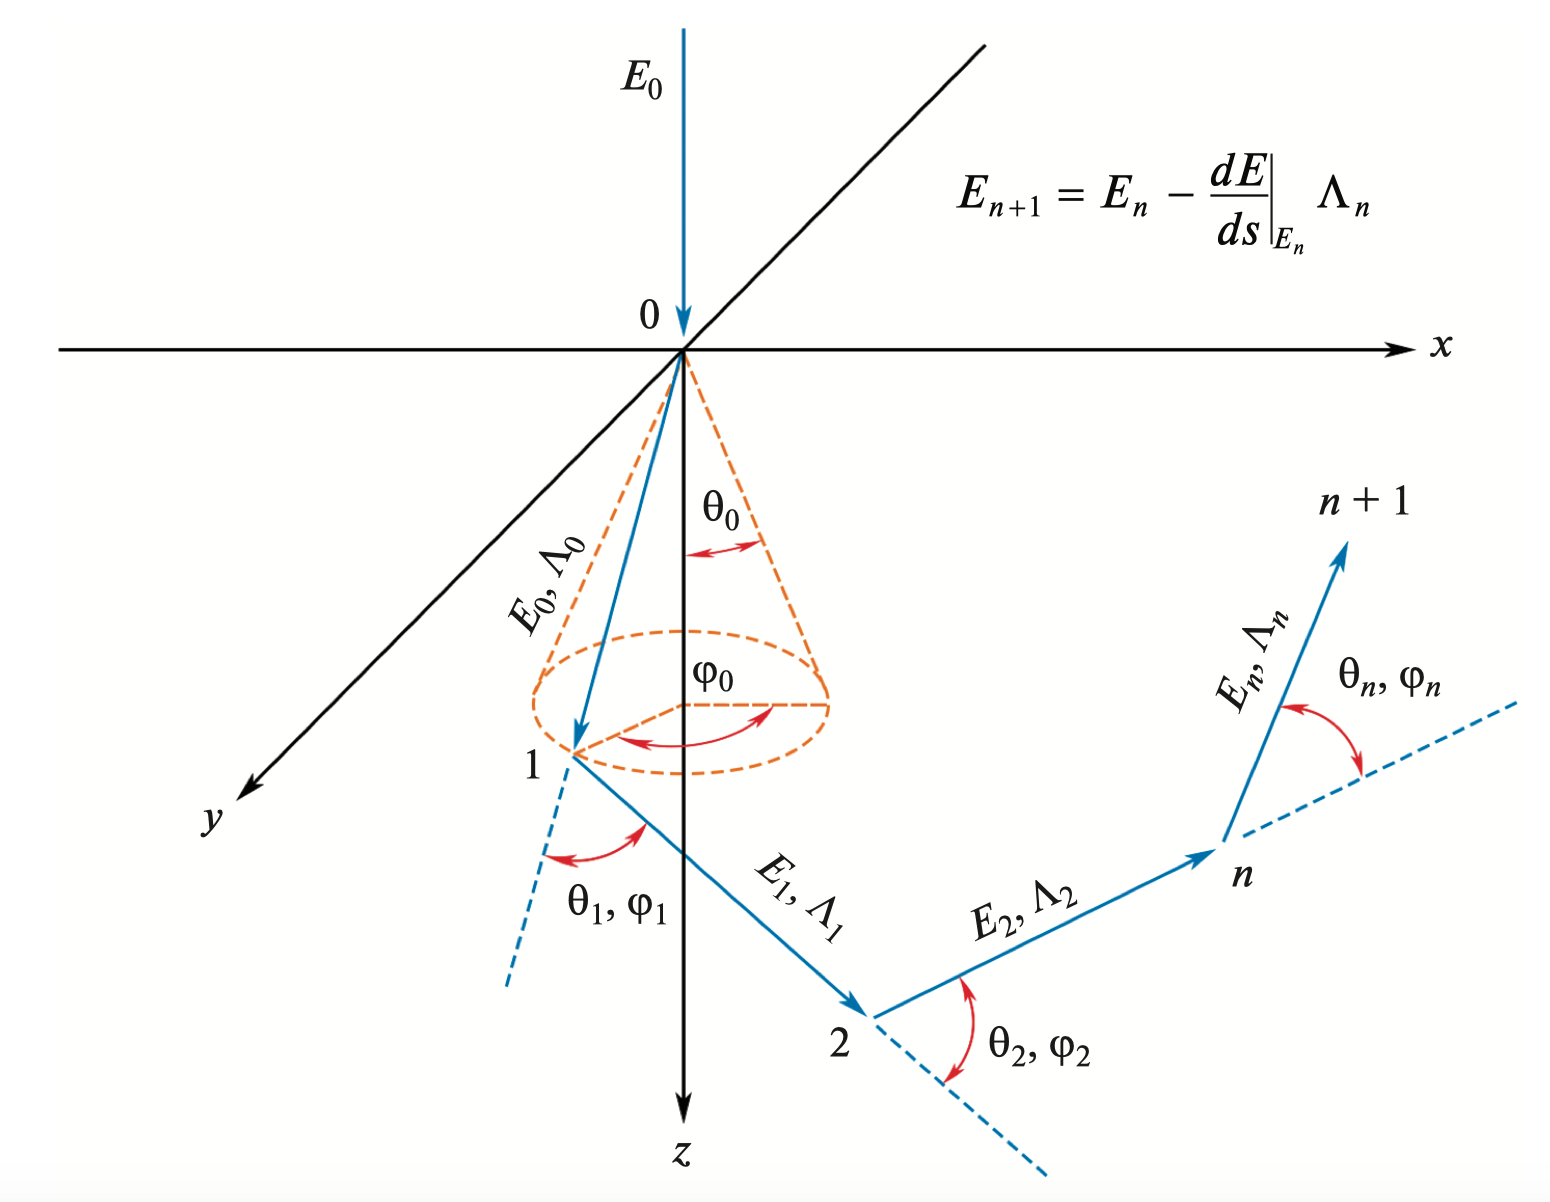
\includegraphics[width=0.8\linewidth]{Monte_Carlo_scheme}
	\caption{Схематическое изображение траектории электрона в веществе, получаемой при Монте-Карло моделировании при использовании модели непрерывных потерь энергии.}
	\label{fig:Monte_Carlo_scheme}
\end{figure}

\section{Моделирование электронно-стимулированных разрывов полимерных молекул}
Количественной характеристикой процесса электронно-стимулированной деградации полимера является радиационно-химический выход разрывов $G_s$, определяемый как число разрывов молекул полимера, происходящее при выделении в нем энергии 100 эВ:
\begin{equation}
	G_s = \frac{N_{scissions}}{100 \text{ эВ}}.
\end{equation}

Экспериментально значение $G_s$ определяется на основе среднечисловых значений молекулярной массы полимера до и после экспонирования ($M_n$ и $M_f$, соответственно), определяемых методом гель-проникающей хроматографии. При известных $M_n$ и $M_f$ значение $G_s$ может быть определено из выражения~\cite{Greeneich1979_Mf_Mn}:
\begin{equation}
	{M_f = \frac{\displaystyle M_n}{1 + \frac{\displaystyle G_s E}{\displaystyle 100 \rho N_A}}}
\end{equation}

Исходя из различных экспериментов по измерению $G_s$, его значение для ПММА при экспонировании электронным лучом было принято равным 1.8~\cite{Charlesby_1964_Gs}. Также было установлено, что при экспонировании гамма- и электронным излучения при различных температурах ($T$) зависимость $\ln G_s (1/T)$ близка к линейной.

Считается, что электронно-стимулированные разрывы полимерных молекул происходят в результате взаимодействия налетающего электрона с валентными электронами атомов углерода, образующими C---C связь в главной цепи ПММА~\cite{Stepanova_2006}.

\begin{narrowfig}{G_value_exp}{G_value_exp}
	Зависимость $G_s$ от T для ПММА при экспонировании гамма- и электронным излучением.
\end{narrowfig}
\subsection{Моделирование термической деполимеризации резиста}
Термическая деполимеризация полимеров включается в себя процессы возникновения активного центра деполимеризации, его распространения вдоль молекулы полимера и последующего затухания или переноса на новую молекулу~\cite{Boyd_1}. Кинетические схемы этих процессов может быть представлена в следующем виде (обозначения $P_n$ и $R_n$ относятся к стабильной полимерной молекуле и радикализованной полимерной молекуле, соответственно, $n$ --степень полимеризации, $R_E$ -- концевой радикал):

\begin{center}
	\textbf{Возникновение активного центра деполимеризации}
	\begin{align*}
		P_n \quad \rightarrow \quad & R_r + R_{n-r} \quad & \text{случайное возникновение} \\
		P_n \quad \rightarrow \quad & R_n + R_E \quad & \text{возникновение на конце молекулы}
	\end{align*}
	\textbf{Распространение активного центра деполимеризации}
	\begin{align*}
		R_n \quad \rightarrow \quad  R_{n-1} + P_1 \qquad\qquad\qquad\qquad\quad\; \text{$P_1$ -- летучий мономер}
	\end{align*}
	\textbf{Перенос активного центра деполимеризации}
	\begin{align*}
		P_n + R_s \quad \rightarrow \quad & P_r + R_{n-r} + P_s
	\end{align*}
	\textbf{Затухание активного центра деполимеризации}
	\begin{align*}
		R_n \quad \rightarrow \quad & P_n \quad & \text{реакция 1 порядка} \\
		R_r + R_s \quad \rightarrow \quad & P_r + P_s \quad & \text{диспропорционирование} \\
		R_r + R_s \quad \rightarrow \quad & P_{r + s} \quad & \text{рекомбинация}
	\end{align*}
\end{center}

На основе данных кинетические схем можно ввести константы вышеописанных процессов и выразить скорость изменения числа стабильных полимерных молекул $P_n$ и радикализованных полимерных молекул $R_n$ за счет каждого из процессов:
\begin{center}
	\textbf{Скорость изменения числа стабильных полимерных молекул $P_n$} \\
	\textit{уменьшения $P_n$ за счет разрывов внутри молекулы:} \\
	$k_s (n-1) P_n$ \\
	\textit{уменьшения $P_n$ за счет разрывов на концах молекулы:} \\
	$k_E P_n$ \\
	\textit{уменьшения $P_n$ за счет переноса активного центра деполимеризации:} \\
	$k_I(R / V)(n-1) P_n$ \\
	\textit{увеличение $P_n$ за счет переноса активного центра деполимеризации:} \\
	{$\displaystyle k_I \frac{R_n}{V} \sum_{n=2}^{\infty} n P_n + k_{\mathrm{r}} \frac{R}{V} \sum_{j=n+1}^{\infty} P_j$} \\
	\textit{увеличение $P_n$ за счет уменьшения числа радикалов:} \\
	$k_T \alpha_n$, $\alpha_n = \left\{
	\begin{array}{l}
		R_n \quad\quad\quad\quad\quad\quad\quad\: \text{реакция 1 порядка} \\
		R_n R / V \quad\quad\quad\quad\quad\: \text{диспропорционирование} \\
		{\displaystyle \frac{1}{2} \sum_{i+j=n}^{\infty} R_i R_j / V} \quad\quad \text{рекомбинация}
	\end{array}\right.,$ \\
	где $R$ -- полное число радикалов: {$\displaystyle R = \sum_{i=1}^{\infty} R_i$} \\
	\textbf{Скорость изменения числа радикализованных полимерных молекул $R_n$} \\
	\textit{увеличение $R_n$ за счет разрывов внутри молекулы:} \\
	$2 k_S \sum_{j=n+1}^{\infty} P_j$ \\
	\textit{увеличение $R_n$ за счет разрывов на концах молекулы:} \\
	$k_E P_n$ \\
	\textit{увеличение $R_n$ за счет распространения активного центра деполимеризации:} \\
	$k_P R_{n+1}$ \\
	\textit{уменьшение $R_n$ за счет распространения активного центра деполимеризации:} \\
	$k_P R_n$ \\
	\textit{увеличение $R_n$ за счет переноса активного центра деполимеризации:} \\
	${\displaystyle k_I \frac{R}{V} \sum_{j=n+1}^{\infty} P_j}$ \\
	\textit{уменьшение $R_n$ за счет переноса активного центра деполимеризации:} \\
	${\displaystyle \frac{k_I R_n}{V} \sum_{n=2}^{\infty} n P_n}$ \\
	\textit{уменьшение $R_n$ за счет уменьшения числа радикалов:} \\
	$k_T \beta R_n$, $\beta = \left\{
	\begin{array}{l}
		1 \quad\quad\quad \text{реакция 1 порядка} \\
		R / V \quad\;\: \text{диспропорционирование или рекомбинация}
	\end{array}\right..$ \\
\end{center}

Учет всех процессов, приводящих к изменению $P_n$ и $R_n$, позволяет описать весь полимерный образец системой уравнений, описывающих каждую степень полимеризации:
\begin{equation} \label{eq:kinetic_system_original}
	\left\{
	\begin{aligned}
		&\dots \\
		&\frac{d P_n}{d t}=-(n-1)\left(k_S+k_I R / V\right) P_n-k_E P_n+k_I R / V \sum_{j=n+1}^{\infty} P_j+k_I R_n \frac{d_0}{m_0}+k_T \alpha_n \\
		&\dots \\
		&\frac{d R_n}{d t}=\left(2 k_S+k_I R / V\right) \sum_{j=n+1}^{\infty} P_j+k_E P_n-\left(\frac{k_I d_0}{m_0}+k_P+k_T \beta\right) R_n+R_P R_{n+1} \\
		&\dots \\
		&\frac{d R_1}{d t}=\left(2 k_S+k_I R / V\right) \frac{W}{x m_0}+\frac{k_E}{m_0} \frac{W}{x}-\left(\frac{k_I d_0}{m_0}+k_T \beta\right) R_1+k_P R_2,
	\end{aligned}
	\right.
\end{equation}
где $m_0$ -- масса мономера, $x$ -- среднечисловая степень полимеризации образца. 

В исходном виде система \ref{eq:kinetic_system_original} включает в себя 2$N$ уравнений ($N$ -- максимальная степень полимеризации молекул образца), и ее решение представляет собой трудоемкую задачу -- не в последнюю очередь за счет суммирования в слагаемых, описывающих эффект переноса активного центра деполимеризации на другую молекулу. Это явление является важной частью процесса полимеризации (в этом случае происходит перенос центра полимеризации)~\cite{chain_transfer_polymerization}, однако его проявление в процессе деполимеризации до сих пор находится под вопросом~\cite{Mita_PMMA_zip_lengths_T}.

Исключение процесса переноса активного центра деполимеризации из рассмотрения, а также предположение о постоянной концентрации радикализованных молекул в слое полимера существенно упрощают систему ~\ref{eq:kinetic_system_original}. В предположении о инициировании деполимеризации за счет разрывов в произвольном месте молекулы она принимает вид~\cite{Boyd_3}:
\begin{equation} \label{eq:Boyd_system_3}
	\left\{
	\begin{aligned}
		&\dots \\
		&d P_n / d t=-(n-1) k_s P_n+k_r R_n \bar{R}, \\
		&\dots \\
		&\dots \\
		&d R_n / d t=2 k_s \sum_{j=n+1}^{\infty} P_j+k_p\left(R_{n+1}-R_n\right)-k_T \bar{R} R_n=0 \quad(n \geq 2) \\
		&\dots \\
		&d R_1 / d t=2 k_s\left(W / x m_0\right)+k_p R_2-k_T \bar{R} R_1=0
	\end{aligned}
	\right.,
\end{equation}
где $\bar{R} = R/V$.

Решение системы~\ref{eq:Boyd_system_3} упрощается при условии, что распределение молекулярной массы полимера является известным. В этом случае преобразования системы приводят ее к совокупности уравнений вида~\cite{Boyd_3}:
\begin{equation} \label{eq:moment_equation}
	\frac{d M_i}{d t}=k_s\left(\frac{2}{i+1}-1\right) M_{i+1}+\frac{d M_0}{d t}-k_s M_1 - \frac{i}{\gamma}\left(k_s M_i+\frac{d M_{i-1}}{d t}\right) \quad(i \geq 1),
\end{equation}
где $1/\gamma = k_p / (k_T \bar{R})$ -- средняя длина цепи деполимеризации, $M_i$ -- момент функции распределения порядка $i$:
\begin{equation}
	M_i=\sum_{n=2}^{\infty} n^i P_n.
\end{equation}

В качестве распределения молекулярной массы полимера может использоваться распределение Шульца-Цимма~\cite{Boyd_3, Schulz-Zimm_distribution}, корректно описывающее полимеры, полученные методом радикальной полимеризации~\cite{Schulz-Zimm_distribution_proof}:
\begin{equation} \label{eq:Schulz-Zimm_distribution}
	P_n = C_0 n^z \exp (-n/y)
\end{equation}
где $P_n$ -- число молекул степени полимеризации $n$, $C_0$ -- нормировочный множитель. Параметр $z$ характеризует ширину распределения:
\begin{equation}
	M_w / M_N=(z+2) /(z+1),
\end{equation}
где $M_n$ и $M_w$ -- среднечисловая и средневесовая молекулярная масса, соответственно, а параметр $y$ определяется из выражения:
\begin{equation}
	x=y(z+1).
\end{equation}

При этом моменты функции распределения высших порядков могут быть выражены через параметры $y$ и $z$ и момент первого порядка $M_1$:
\begin{equation}
	M_i=M_1 \prod_{n=2}^i(z+n) y^{i-1}.
\end{equation}
Отметим, что $M_0$ выражает полное число полимерных молекул, $M_1$ -- среднечисловую степень полимеризации.

Далее удобно ввести безразмерные переменные:
\begin{equation}
	\begin{aligned}
		\tau & = y^0 k_s t \\
		\tilde{M}_1 & = M_1 / M_1^0 \\
		\tilde{y} & = y / y^0 \\
		\tilde{\gamma} & = \gamma y^0 \\
		\tilde{x} & = x / x^0 = \left[y(z+1) / y^0\left(z^0+1\right)\right],
	\end{aligned}
\end{equation}
которые в дальнейшем используются в уравнениях вида~\ref{eq:moment_equation} для $i$, равного 1, 2 и 3. В конечном счете система этих трех нелинейных дифференциальных уравнений первого порядка принимает вид:

\begin{equation} \label{eq:scary_system}
	\begin{aligned}
		&\frac{\tilde{M_1}^{\prime}}{\tilde{M_1}}=\left[\frac{1}{\tilde{y}} \frac{d \tilde{y}}{d \tau}+\frac{1}{(z+1)} \frac{d z}{d \tau}-\tilde{y}(z+1)\right] /[1+\tilde{\gamma} \tilde{y}(z+1)] \\
		&\tilde{y}^{\prime}=(B F-C E) /(A E-D B) \\
		&z^{\prime}=(C D-A F) /(A E-D B),
	\end{aligned}
\end{equation}
где
\begin{equation}
	\begin{aligned}
		&A=-\left[\frac{1}{\tilde{y}[1+\tilde{\gamma} \tilde{y}(z+1)]}+\frac{(z+2) \tilde{\gamma}}{(z+2) \tilde{\gamma} \tilde{y}+2}\right] \\
		&B=-\left[\frac{1}{(z+1)[1+\tilde{\gamma} \tilde{y}(z+1)]}+\frac{\tilde{\gamma} \tilde{y}}{(z+2) \tilde{\gamma} \tilde{y}+2}\right] \\
		&C=\left[\frac{\tilde{y}(z+1)}{\tilde{\gamma} \tilde{y}(z+1)+1}-\frac{\frac{1}{3}(z+2)(z+3) \tilde{\gamma} \tilde{y}^2+2(z+2) \tilde{y}}{(z+2) \tilde{\gamma} \tilde{y}+2}\right] \\
		&D=\left[\frac{(z+2) \tilde{\gamma}}{(z+2) \tilde{\gamma} \tilde{y}+2}-\frac{2(z+2)(z+3) \tilde{\gamma} \tilde{y}+3(z+2)}{(z+2)(z+3) \tilde{\gamma} \tilde{y}^2+3(z+2) \tilde{y}}\right] \\
		&E=\left[\frac{\tilde{\gamma} \tilde{y}}{(z+2) \tilde{\gamma} y+2}-\frac{\tilde{\gamma} \tilde{y}(2 z+5)+3}{(z+2)(z+3) \tilde{\gamma} \tilde{y}+3(z+2)}\right] \\
		&F=\left[\frac{\frac{1}{3}(z+2)(z+3) \tilde{\gamma} \tilde{y}^2+2(z+2) \tilde{y}}{(z+2) \tilde{\gamma} \tilde{y}+2}-\right. \\
		&\left.-\frac{\frac{1}{2}(z+2)(z+3)(z+4)\left(\tilde{\gamma} \tilde{y}^2+3(z+2)(z+3) \tilde{y}\right.}{(z+2)(z+3) \tilde{\gamma} \tilde{y}+3(z+2)}\right].
	\end{aligned}
\end{equation}
Производные в левой части~\ref{eq:scary_system} берутся по переменной $\tau$, а сама система решается численно.
\section{Диффузия мономера в слое полимера}
Ключевая величина, описывающая в процесс диффузии произвольной примеси в слое вещества -- коэффициент диффузии. В настоящее время существуют два основных подхода к определению коэффициента диффузии мономера ММА в слое ПММА. Первый из них основан на использовании теории свободного объема, что позволяет непосредственно определить коэффициент диффузии на основе различных параметров вещества. Второй подход основан на косвенном определении коэффициента диффузии за счет моделирования выхода мономера из слоя ПММА и сравнения результатов моделирования с экспериментальными данными.

\subsection{Теория свободного объема}
Точный расчет коэффициента диффузии возможен на основе теории свободного объема~\cite{Vrentas_free_volume, Zielinski_free_volume}, что требует задания большого числа параметров:
\begin{equation}
	\ln D=\ln \bar{D}_0-\frac{E^*}{\mathrm{R} T}-\left\{\frac{\left(1-\omega_2\right) \hat{V}_1^*+\xi \omega_2 \hat{V}_2^*}{\hat{V}_{\mathrm{FH}} / \gamma}\right\}.
\end{equation}
Здесь $\bar{D}_0$ -- константа, $E^*$ -- энергия на моль частиц примеси, необходимая для преодоления сил притяжения, $R$ -- универсальная газовая постоянная, $T$ -- температура, $\xi$ и $\gamma$ -- параметры, $\hat{V}_1^*$ и $\hat{V}_2^*$ -- удельные объемы вещества и примеси, соответственно, $\hat{V}_{\mathrm{FH}}$ -- средний свободный объем полостей в смеси вещества и примеси, $\omega_2$ -- массовая доля полимера в смеси ($w_p$). Величина $\hat{V}_{\mathrm{FH}} / \gamma$ определяется выражением
\begin{equation}
	\hat{V}_{\mathrm{FH}} / \gamma=\left(1-\omega_2\right)\left(\frac{K_{11}}{\gamma_1}\right)\left(K_{21}+T-T_{\mathrm{g} 1}\right)+\omega_2 \hat{V}_{\mathrm{FH} 2} / \gamma_2,
\end{equation}
где $\left(K_{11} / \gamma_1\right)$ и $\left(K_{21}-T_{\mathrm{g} 1}\right)$ -- параметры примеси, величина $\hat{V}_{\mathrm{FH} 2} / \gamma_2$ описывает вклад полимерной матрицы в средний свободный объем полостей. Эта величина зависит от того, находится система выше или ниже температуры стеклования полимера ($T_{g2}$):
\begin{equation}
	\begin{aligned}
		&\hat{V}_{FH2} =
		\hat{V}_2^0 (T_{g2}) \left[ f_{H2}^{G}+\alpha_2 (T-T_{g2}) \right], & T \geq T_{g2} \\
		&\hat{V}_{FH2} =
		\hat{V}_2^0 (T_{g2})\left[f_{H2}^{G}+(\alpha_2-\alpha_{c2})(T-T_{g2})\right], \hspace{1em} & T<T_{g2}
	\end{aligned}
\end{equation}
В этом выражении $\hat{V}_2^0\left(T_{\mathrm{g} 2}\right)$ -- удельный объем полимера при температуре $T_{g2}$, \linebreak $\alpha_2$ -- коэффициент температурного расширения полимера в состоянии равновесия, $f_{\mathrm{H} 2}^{\mathrm{G}}$ -- доля объема пустот в полимере при температуре $T_{g2}$:
\begin{equation}
	f_{\mathrm{H} 2}^{\mathrm{G}}=\alpha_2 K_{22},
\end{equation}
\begin{equation}
	\alpha_{\mathrm{c} 2}=\frac{1}{T_{\mathrm{g} 2}} \ln \left(\frac{\hat{V}_2^0\left(T_{\mathrm{g} 2}\right)\left(1-f_{\mathrm{H} 2}^{\mathrm{G}}\right)}{\hat{V}_2^0(0)}\right),
\end{equation}
\begin{equation}
	\gamma_2=\frac{\hat{V}_2^0\left(T_{\mathrm{g} 2}\right) \alpha_2}{\left(K_{12} / \gamma_2\right)},
\end{equation}
\begin{equation}
	\hat{V}_1^*=\hat{V}_1^0(0); \hspace{1em} \hat{V}_2^*=\hat{V}_2^0(0),
\end{equation}
где $K_{22}$ и $\left(K_{12} / \gamma_2\right)$ -- параметры модели свободного объема, $\hat{V}_1^0(0)$ и $\hat{V}_2^0(0)$ -- удельные объемы примеси и полимера в состоянии равновесия при $T=0$K. Параметры модели свободного объема для диффузии ММА в слое ПММА приведены в таблице~\ref{table:D_free_volume}~\cite{Tonge_free_volume_parameters}.

\begin{table}[h]
	\centering
	\caption{Константы процессов инициирования активного центра и деполимеризации.}
	\begin{tabular}{l c l}
		\hline \hline
		Параметр & \hspace{4em} & Значение \\ \hline
		$\hat{V}_1^0(0)$, см$^{-1}$ & \hspace{1em} & 0.871 \\
		$\tilde{V}_1^0(0)$, см$^3$ моль$^{-1}$ & \hspace{1em} & 86.9 \\
		$\hat{V}_2^0(0)$, см$^3$ г$^{-1}$ & \hspace{1em} & 0.762 \\
		$\tilde{V}_2^*$, см$^3$ моль$^{-1}$ & \hspace{1em} & 135 \\
		$f_{H2}^{G}$ & \hspace{1em} & 0.00456 \\
		$K_{22}$, К & \hspace{1em} & 80 \\
		$(K_{12} / \gamma_2)$, см$^3$ г$^{-1}$ К$^{-1}$ & \hspace{1em} & 1.28$\times$10$^{-4}$ \\
		$\gamma_2$ & \hspace{1em} & 3.88 \\
		$\alpha_{c2}$, K$^{-1}$ & \hspace{1em} & 2.37$\times$10$^{-4}$ \\
		$\xi_L$ & \hspace{1em} & 0.64 \\
		$\xi$ & \hspace{1em} & 0.58 \\
		$E^*$, Дж моль$^{-1}$ & \hspace{1em} & 0.58 \\
		$\bar{D}_0$, см$^2$ с$^{-1}$ & \hspace{1em} & 1.27$\times$10$^{-3}$ \\
		$(K_{11} / \gamma_1)$, см$^3$ г$^{-1}$ К$^{-1}$ & \hspace{1em} & 6.91$\times$10$^{-4}$ \\
		$(K_{21}-T_{g1})$, К & \hspace{1em} & 72.26 \\
		$\hat{V}_2^0(T_{g2})$, см$^3$ г$^{-1}$ & \hspace{1em} & 0.8754 \\
		$\tilde{V}_c$, см$^3$ моль$^{-1}$ & \hspace{1em} & 311 \\
		\hline \hline
	\end{tabular}
	\label{table:D_free_volume}
\end{table}

Результаты применения модели свободного объема для вычисления коэффициента диффузии ММА в ПММА приведены на рис.~\ref{fig:free_volume_diffusion}

\begin{figure}
	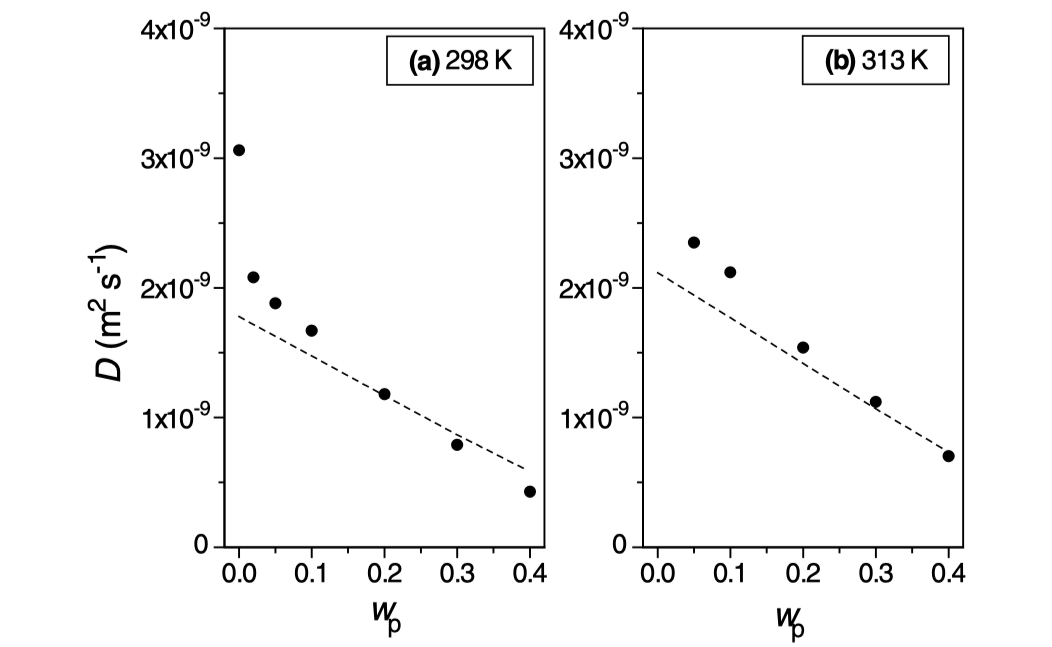
\includegraphics[width=0.9\linewidth]{free_volume_diffusion}
	\caption{Результаты применения модели свободного объема для вычисления коэффициента диффузии ММА в ПММА при 296 К (а) и 313 К (б): пунктирная линия -- рассчитанные значения, точки -- экспериментальные значения~\cite{Griffiths_MMA_PMMA_diffusion}.}
	\label{fig:free_volume_diffusion}
\end{figure}


\subsection{Вычисление коэффициента диффузии на основе модели выхода мономера из слоя полимера}
В работе~\cite{Fragala_3_diffusion} проводилось исследование выхода мономера из слоя ПММА при его экспонировании ионным лучом. В модели процесса деполимеризации ПММА рассматривались процессы инициирования активного центра деполимеризации и распространения активного центра деполимеризации вдоль молекулы:

\begin{equation}
	\begin{aligned}
		&{[\text { Полимер }]_N \stackrel{\text { Экспонирование }}{\longrightarrow}[\text { Полимер }]_{N-m}+[\text { Радикал }]_m,} \\
		&{[\text { Радикал }]_m \stackrel{\text { Деполимеризация }}{\longrightarrow} \text { Мономер }+[\text { Радикал }]_{m-1} .}
	\end{aligned}
\end{equation}
$K_i$ и $K_p$.
Концентрация центров инициирования деполимеризации ($c_I$) описывалась уравнением
\begin{equation}
	\frac{\partial c_I}{\partial t}=K_i f(t)-K_p c_I,
\end{equation}
где $K_i$ и $K_p$ -- константы процессов инициирования и деполимеризации, а функция $f(t)$ описывает режим работы ионного луча:
\begin{equation}
	f(t) = 1 - H(t - t_0),
\end{equation}
где $H(t)$ -- функция Хевисайда,  $t_0$ -- время работы ионного луча.

Образование мономера предполагалось однородным по объему полимера, что позволило описать процесс выхода мономера одномерным уравнением диффузии:
\begin{equation} \label{eq:raduino_diff_eq}
	\frac{\partial c_M}{\partial t}=D\left(\frac{\partial^2 c_M}{\partial z^2}\right)+\beta K_p c_I,
\end{equation}
где $c_M$ -- концентрация мономера, $D$ -- коэффициент диффузии мономера в слое ПММА, считающийся постоянным по всему объему слоя, $\beta$ -- количество мономеров, образующихся при инициирования активного центра деполимеризации.

Уравнение~\ref{eq:raduino_diff_eq} дополнялось начальными и граничными условиями, описывающими беспрепятственный переход мономера через границу ПММА/вакуум, отражение мономера от подложки и его отсутствие до и по истечении большого времени после работы ионного луча, имели вид:
\begin{equation} \label{eq:diff_eq_conditions}
	\begin{aligned}
		&\left.c_M\right|_{z=z_0}=0, \\
		&\left.\frac{\partial c_M}{\partial z}\right|_{z=0}=0, \\
		&\left.c_M\right|_{t=0}=0, \\
		&\lim _{t \rightarrow \infty} c_M=0, \\
		&\lim _{t \rightarrow \infty} c_I=0,
	\end{aligned}
\end{equation}
где $z = 0$ и $z = z_0$ -- границы слоя ПММА.

Решение уравнения~\ref{eq:raduino_diff_eq} с условиями~\ref{eq:diff_eq_conditions} позволило рассчитать поток мономера через границу полимер/вакуум во время работы ионного луча ($t < t_0$):
\begin{equation}
	\begin{aligned}
		J_{+}(t)= & A \beta K_i z_0
		\left[
		1-\frac{8}{\pi^2} \sum_{n=1}^{\infty}
		\frac{1}{(2n-1)^2} \frac{1}{(1-\alpha_n / K_p)} \times \right. \\ & \left.
		\times
		\left(
			\exp (-\alpha_n t)-\frac{\alpha_n}{K_p} \exp (-K_p t)
		\right)
		\right]
	\end{aligned}
\end{equation}
и после выключения ионного луча ($t > t_0$):
\begin{equation}
	\begin{aligned}
		J_{-}(t)= A \beta K_i z_0 \left[
			\frac{8}{\pi^2} \sum_{n=1}^{\infty} \frac{1}{(2 n-1)^2} \frac{1}{\left(1-\alpha_n / K_p\right)}\right. \times \quad \quad \quad \quad \\
	\times \left.
	\left(
	\exp (-\alpha_n t) (\exp (\alpha_n t_0)-1)- \frac{\alpha_n}{K_p}
	\exp (-K_p t) (\exp (K_p t_0)-1)
	\right)
	\right].
	\end{aligned}
\end{equation}

Параметры модели $K_i$, $K_p$ и $\beta$ были подобраны за счет сравнения промоделированной зависимости потока мономера от времени с экспериментальной, их значения приведены в таблице~\ref{table:Ki_Kp_D}.

\begin{figure}
	\begin{minipage}{0.48\textwidth}
		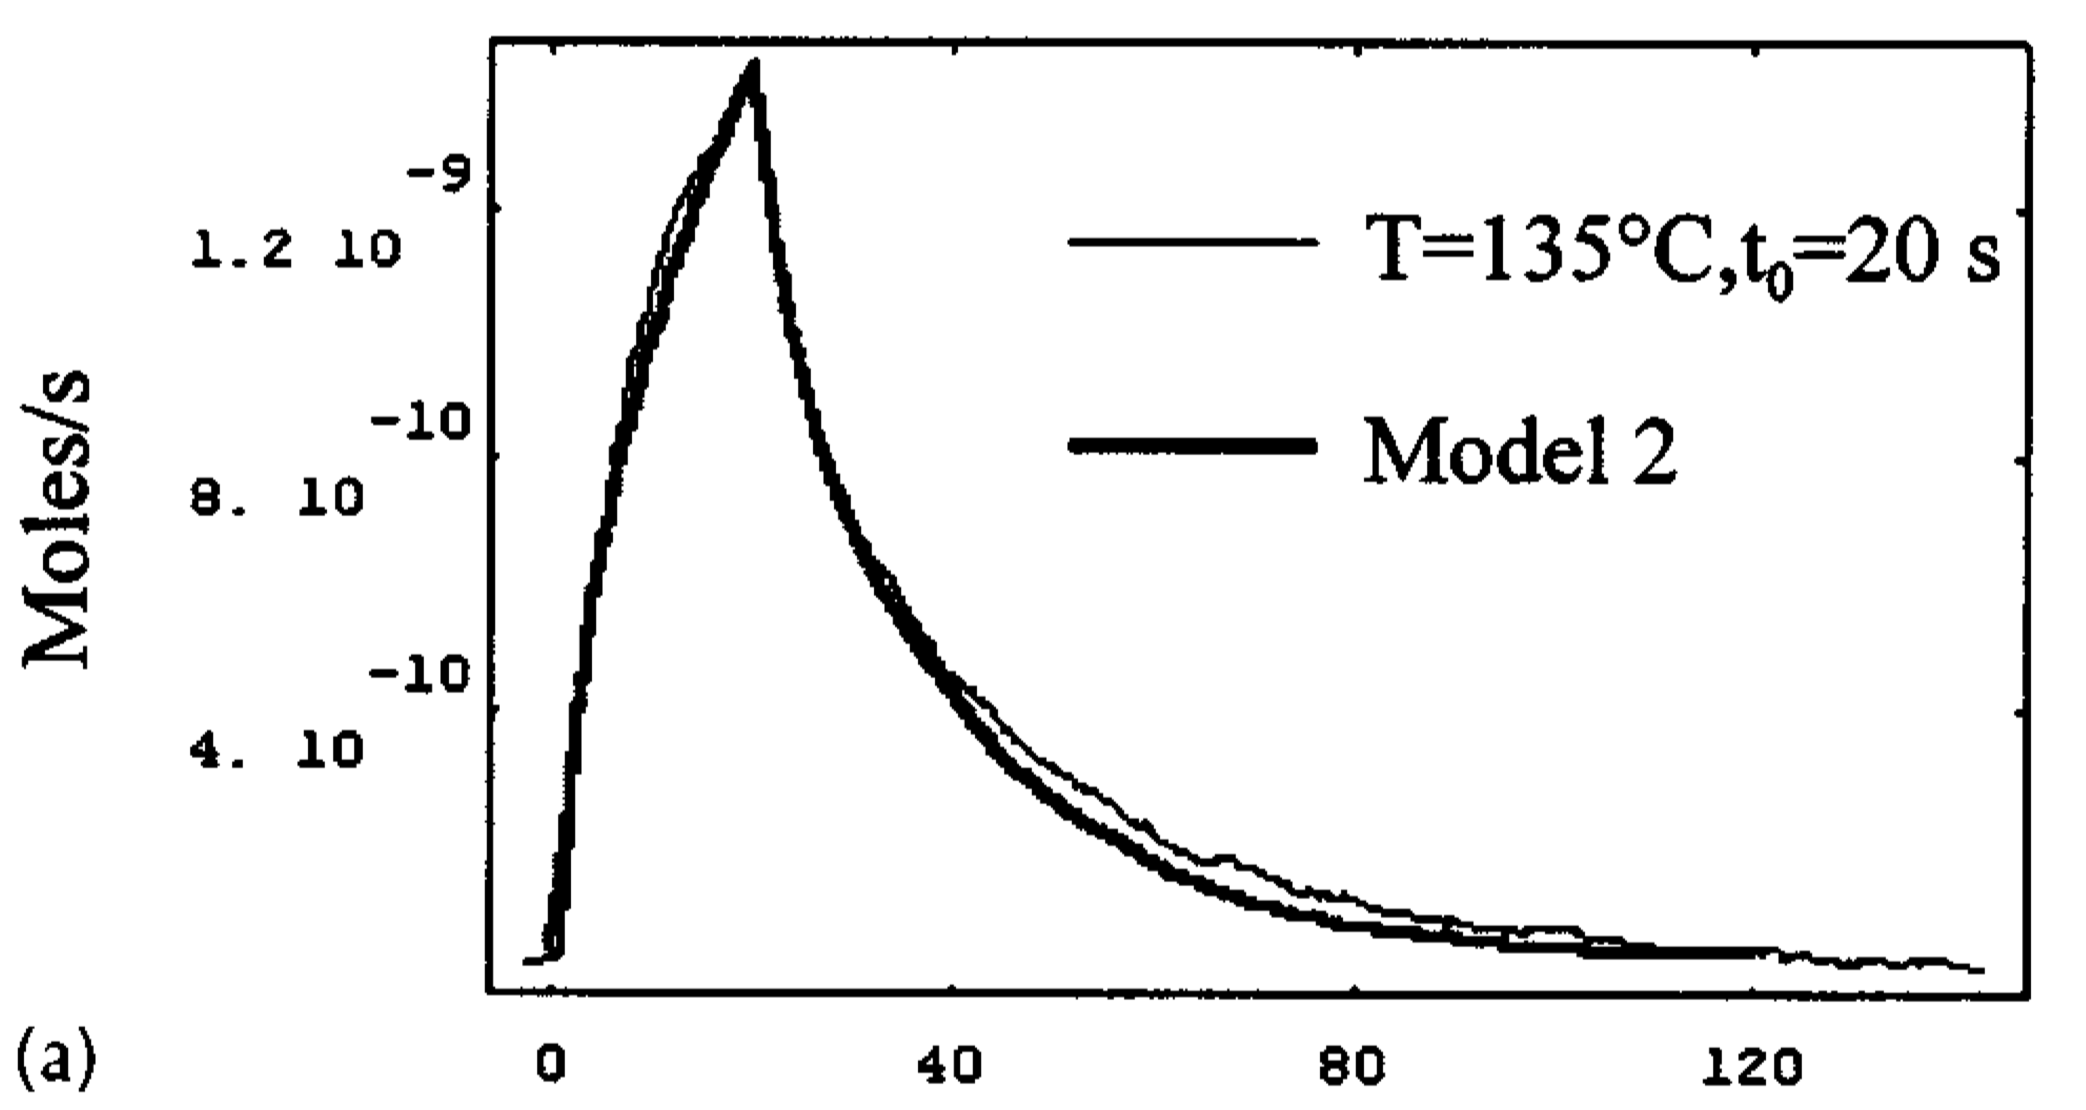
\includegraphics[width=\linewidth]{135_20.png}
	\end{minipage}
	\begin{minipage}{0.48\textwidth}
		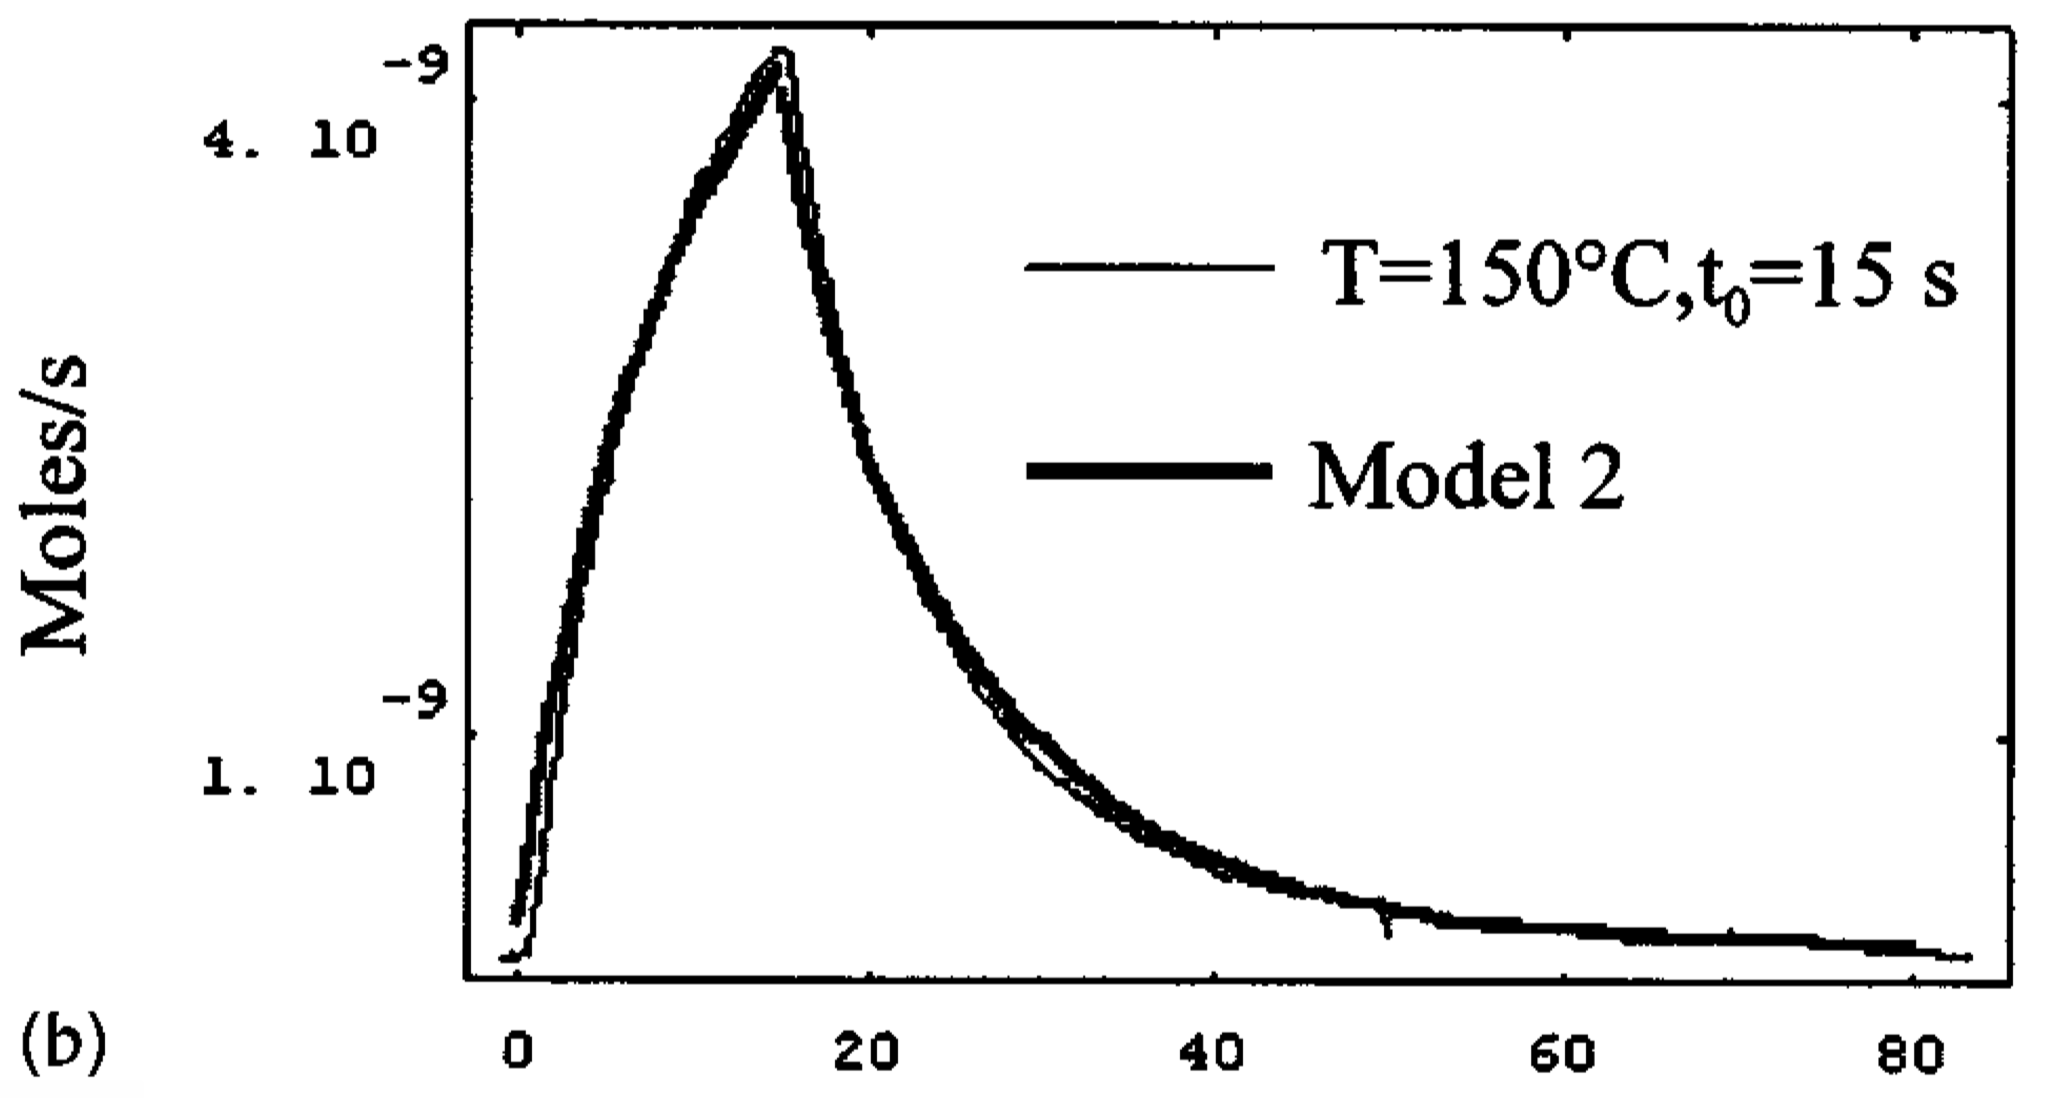
\includegraphics[width=\linewidth]{150_15.png}
	\end{minipage}
	\caption{Экспериментальная зависимость скорости выхода мономера из слоя ПММА при экспонировании ионным лучом и результаты моделирования, полученные в работе для температур 135$^\circ$C и 150$^\circ$C~\cite{Fragala_3_diffusion}}
\end{figure}

\begin{table}[h]
	\begin{center}
	\caption{Константы процессов инициирования активного центра и деполимеризации и коэффициенты диффузии, полученные в работе~\cite{Fragala_3_diffusion} для различных температур.}
	\begin{tabular}{lc rc rc r}
		\hline \hline
		Температура, $^\circ$C & \hspace{4em} & $K_i \beta$, с$^{-1}$ & \hspace{1em} & $K_p$, с$^{-1}$ & \hspace{1em} & $D$, см$^2$с$^{-1}$ \\ \hline
		135 & \hspace{4em} & $7 \times 10^{-4}$ & \hspace{1em} & 90 & \hspace{1em} & $2 \times 10^{-10}$ \\  
		150 & \hspace{4em} & $1.85 \times 10^{-3}$ & \hspace{1em} & 100 & \hspace{1em} & $3.5 \times 10^{-10}$ \\
		160 & \hspace{4em} & $1.6 \times 10^{-3}$ & \hspace{1em} & 100 & \hspace{1em} & $1.1 \times 10^{-9}$ \\
		170 & \hspace{4em} & $3.2 \times 10^{-3}$ & \hspace{1em} & 120 & \hspace{1em} & $1.2\times10^{-9}$ \\
		185 & \hspace{4em} & $3.1 \times 10^{-3}$ & \hspace{1em} & 300 & \hspace{1em} & $2.1\times10^{-9}$ \\ \hline \hline
	\end{tabular}
	\label{table:Ki_Kp_D}
	\end{center}
\end{table}

\section{Моделирование термического растекания резиста}


\subsection{Аналитический подход}
Моделирование оплавления резиста может быть проведено аналитически на основе подхода, предложенного для моделирования оплавления периодических структур, полученных методом НИЛ~\cite{Leveder_2008, Leveder_2011}. В его основе лежит Фурье-преобразование профиля резиста $h(t)$:
\begin{equation}
	\begin{aligned}
		& h(x, t) = h_0 + \tilde{h}(x, t) \\
		& \tilde{h}(x, t) = \sum_{-\infty}^{+\infty} a_n(t) \exp \left(i n \frac{2 \pi}{\lambda} x\right),
	\end{aligned}
\end{equation}
где $h_0$ -- средняя высота профиля, $\lambda$ -- пространственный период профиля.

Уравнения Навье-Стокса при условии отсутствия проскальзывания и с учетом расклинивающего и Лапласова давления может быть выражено в виде:
\begin{equation}
	\partial_t \tilde{h}-\frac{A}{6 \pi \eta h_0} \partial_x^2 \tilde{h}+\frac{\gamma h_0^3}{3 \eta} \partial_x^4 \tilde{h} = 0,
\end{equation}
где $A$ -- постоянная Гамакера, $\gamma$ -- коэффициент поверхностного натяжения резиста.

Его решение приводит к выражению для времени затухания $n$-й гармоники профиля $\tau_n$:
\begin{equation}
	\frac{1}{\tau_n}=\left(n \frac{2 \pi}{\lambda}\right)^2 \frac{A}{6 \pi h_0 \eta}+\left(n \frac{2 \pi}{\lambda}\right)^4 \frac{\gamma h_0^3}{3 \eta}.
\end{equation}

При выполнении условия $\left(\frac{\displaystyle h_0^2}{\displaystyle \lambda}\right)^2 \ll \frac{\displaystyle A}{\displaystyle \gamma}$ выражение для $\tau_n$ принимает более простой вид:
\begin{equation}
	\tau_n=\frac{3 \eta}{\gamma h_0^3} \times\left(\frac{\lambda}{2 \pi n}\right)^4.
\end{equation}

Результирующий профиль в момент времени $t$ определяется суммой гармоник:
\begin{equation}
	\tilde{h}(x, t)=\sum_{-\infty}^{+\infty} a_n(0) \exp \left(-\frac{t}{\tau_n}+i n \frac{2 \pi}{\lambda} x\right).
\end{equation}

\begin{figure}
	\begin{center}
		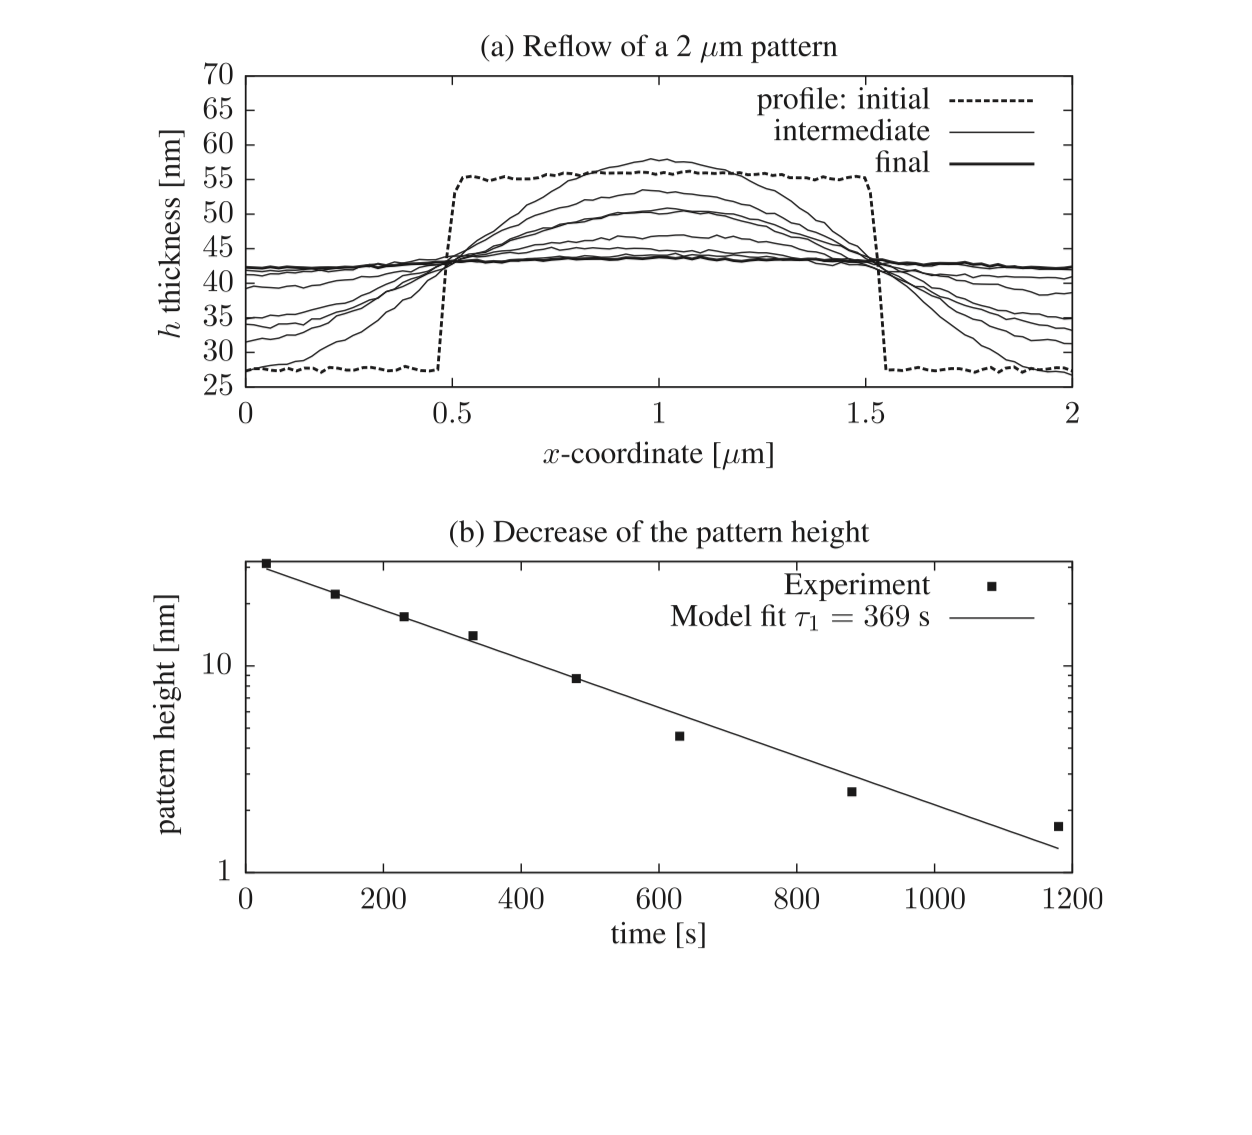
\includegraphics[width=0.6\linewidth]{reflow_analytical}
		\caption{Растекание решетки с периодом 2 мкм, полученной в ПММА методом наноимпринтной литографии~\cite{Leveder_2011}. Нагрев производился при температуре 145 $^\circ$С, время нагрева составляло от 50 до 1200 с: а) 2D профили, полученные методом атомно-силовой микроскопии, б) зависимость от времени высоты профиля решетки (точки) и подгонка линейной функцией (сплошная линия).}
		\label{fig:ferlow_analytical}
	\end{center}
\end{figure}


\subsection{Численный подход}
Второй подход к моделированию растекания профиля резиста основан на использовании численного метода конечных элементов, реализованном в программе \textquotedbl Surface Evolver\textquotedbl{}~\cite{Brakke_SE}. В этом подходе структурные свойства трехмерного объекта задаются свойствами его поверхности, и эволюция формы объекта в различных процессах описываются изменением формы его поверхности. При этом объем внутри поверхности на протяжении процесса эволюции формы поддерживается постоянным. В процессе моделирования поверхность объекта разбивается на треугольные площадки -- грани, задаваемыми тремя узлами -- вершинами, которые, в свою очередь, соединяются ориентированными ребрами~\ref{fig:SE_12}.

В процессе моделирования эволюции формы объекта производится на основе минимизации полной поверхностной энергии. Энергия отдельной грани вычисляется по формуле
\begin{equation}
	E_i=\frac{\gamma_i}{2}\left\|\vec{e}_0 \times \vec{e}_1\right\|,
\end{equation}
где $\gamma_i$ -- коэффициент поверхностного натяжения грани с номером $i$. Сила, действующая на вершину $V_0$ (рис.~\ref{fig:SE_12}), определяется выражением
\begin{equation}
	\vec{F}_{V_0}=\frac{T}{2} \cdot \frac{\vec{e}_1 \times\left(\vec{e}_0 \times \vec{e}_1\right)}{\left\|\vec{e}_0 \times \vec{e}_1\right\|}.
\end{equation}

При моделировании растекания двумерных структур в резисте последние представляются в виде фигуры бесконечной протяженность. При этом моделирование проводится для участка фигуры конечной длины с использованием зеркальных граничных условия на краях участка~\ref{fig:SE_3}. Таким образом, возникают три возможных типа граней -- грани на границе полимер/вакуум ($p$), грани на границе полимер/подложка ($ps$) и боковые (зеркальные) грани ($m$). Полная энергия поверхности $E_{tot}$ вычисляется по формуле
\begin{equation}
	E_{tot}=E_p-(E_{p s}+E_m),
\end{equation}
где 
\begin{equation}
	E_x = \sum_{i} E_{x,i}, \hspace{0.5em} x = p, ps, m
\end{equation}

\begin{figure}
	\begin{minipage}{0.55\textwidth}
		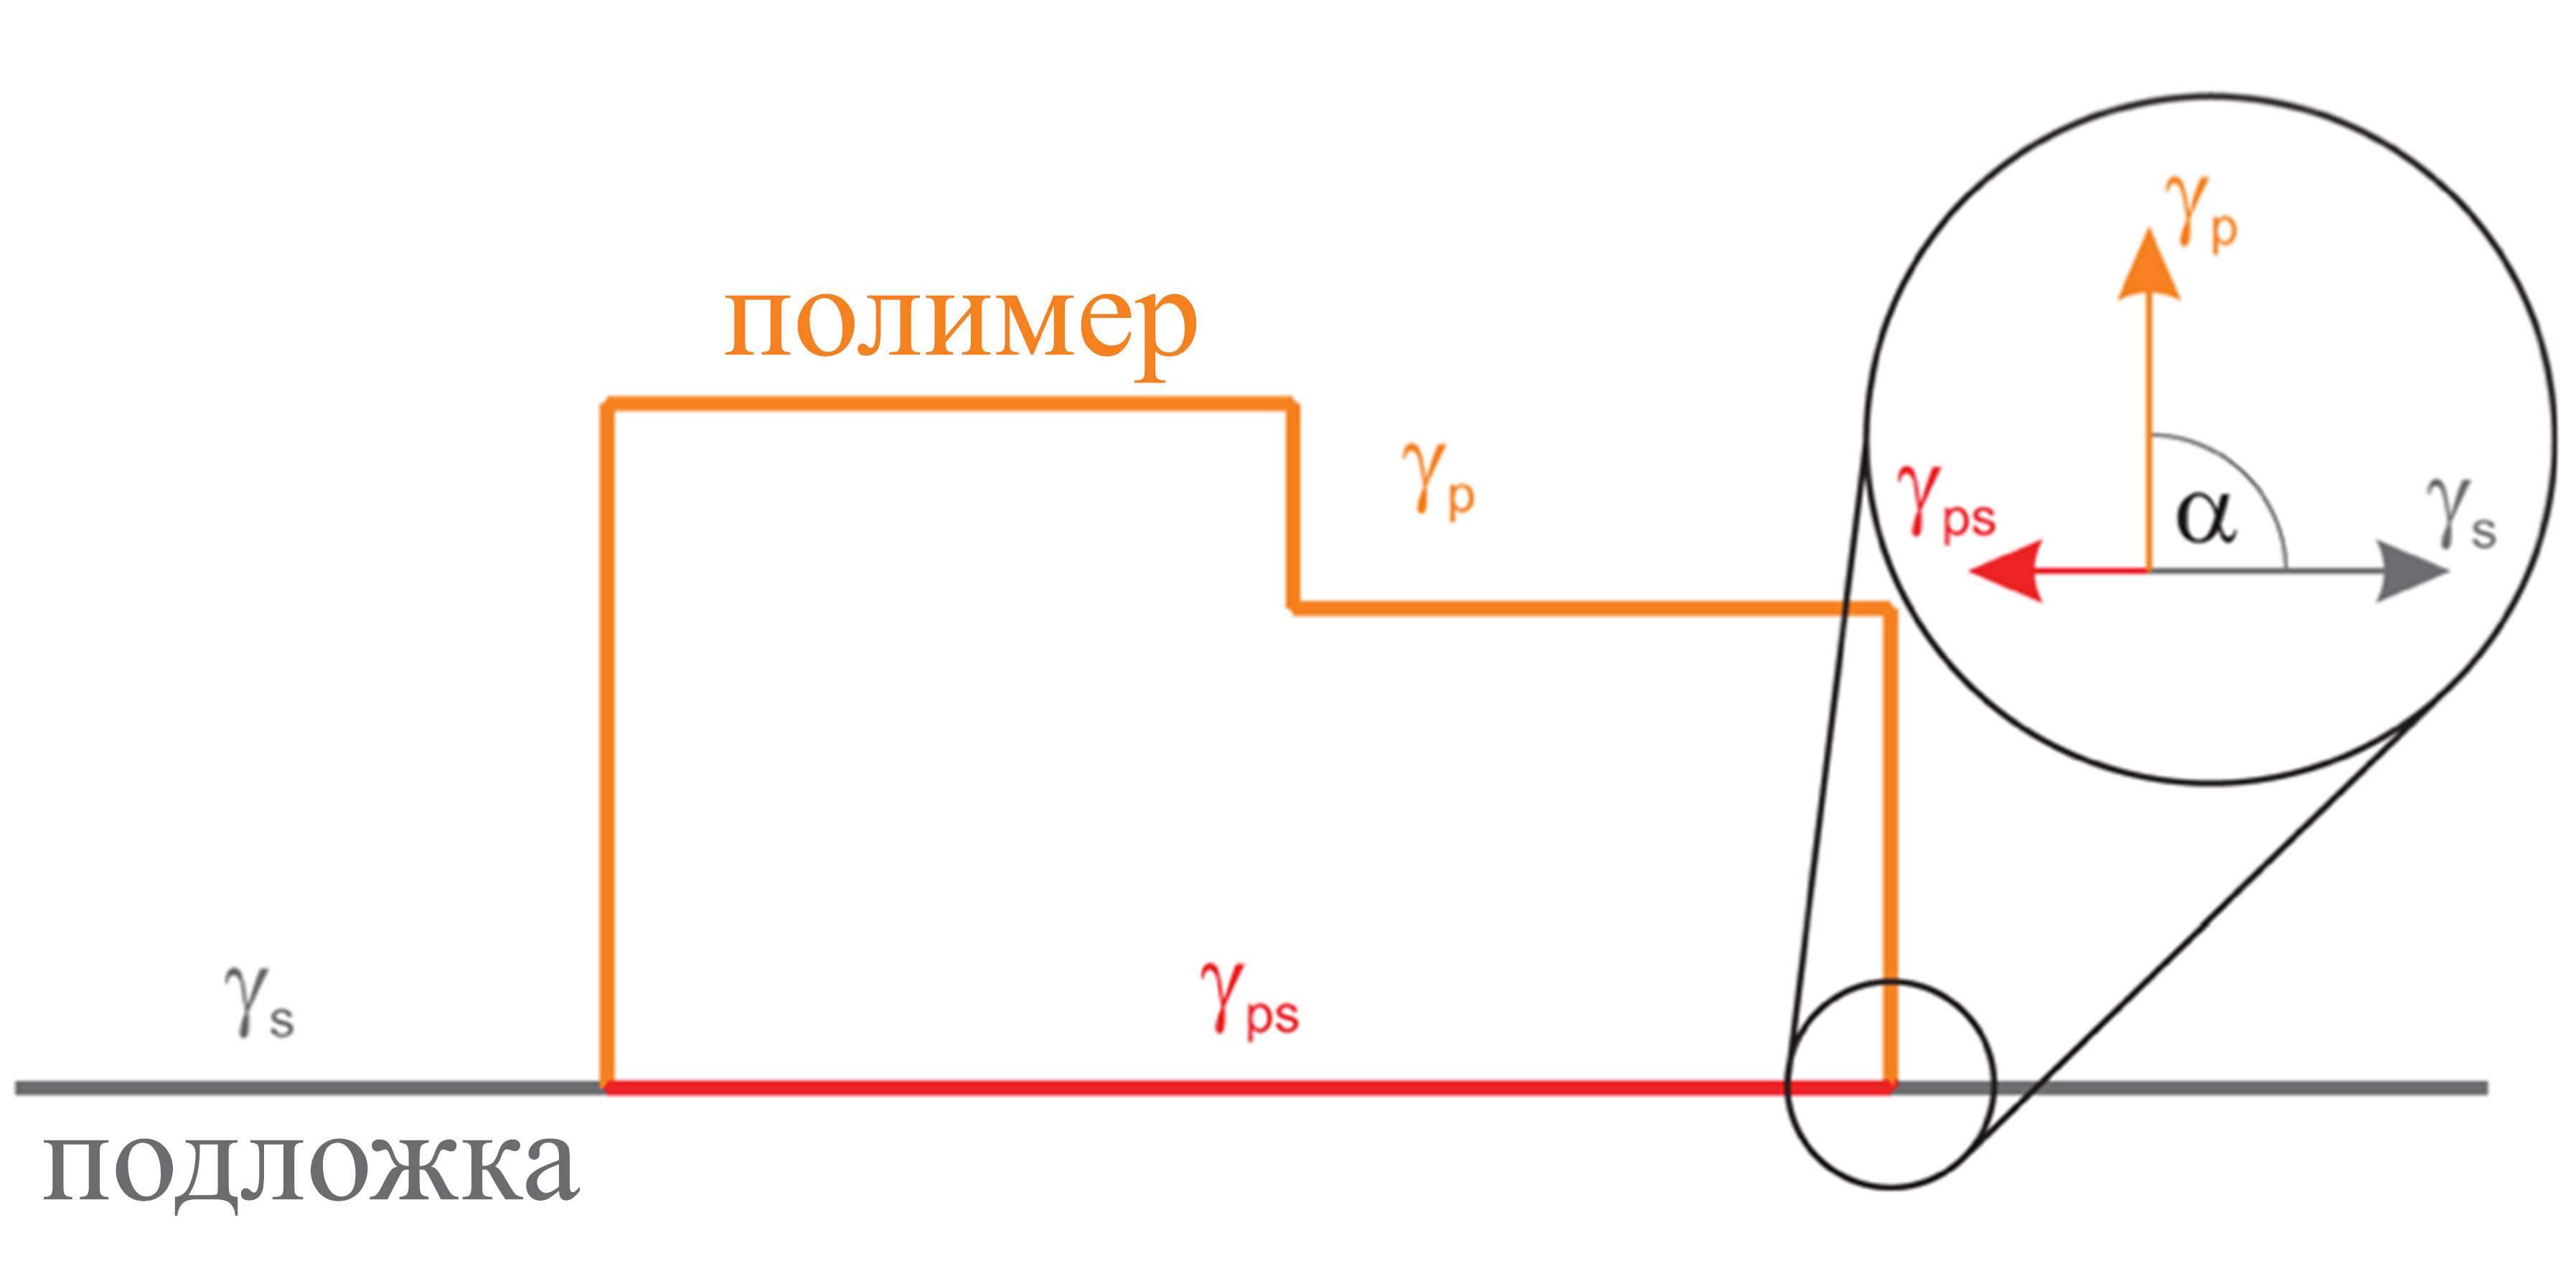
\includegraphics[width=\linewidth]{SE_1}
	\end{minipage}
	\begin{minipage}{0.4\textwidth}
		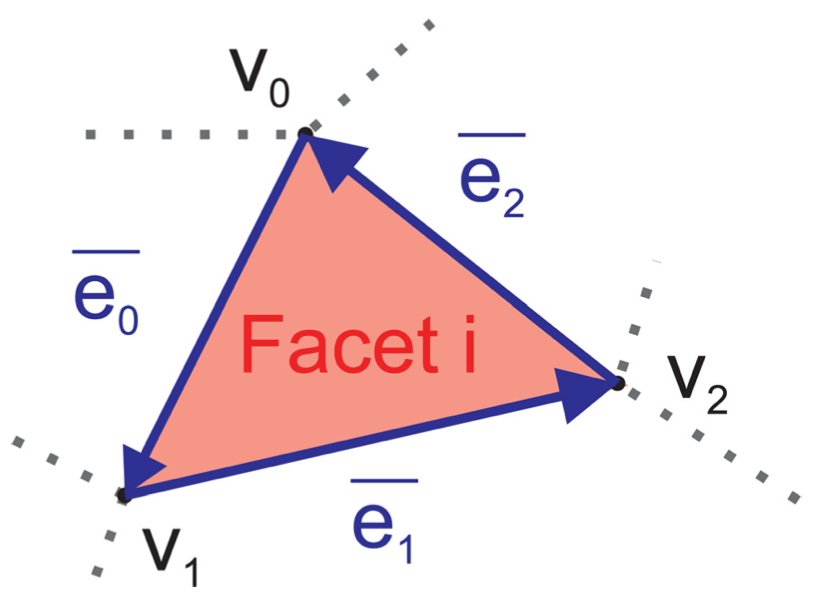
\includegraphics[width=\linewidth]{SE_2}
	\end{minipage}
	\caption{Схематическое изображение поверхности в программе \textquotedbl Surface Evolver\textquotedbl{}}.
	\label{fig:SE_12}
\end{figure}

В работах по использованию программы \textquotedbl Surface Evolver\textquotedbl{} для моделирования растекания слоя ПММА моделирование проводилось в режиме нормализации площади, использующимся для реалистичного описания движения под действием сил поверхностного натяжения. В этом режиме при вычислении силы, действующей на вершину, учитывается площадь всех граней, окружающих вершину. Поскольку каждая из граней задается тремя вершинами,
сила, действующая на каждую из вершин грани, будет пропорциональна отношению площади грани к 1/3 площади всех граней, окружающих данную вершину ($A$):
\begin{equation}
	\vec{F}_{norm} = \frac{\vec{F}}{A/3} = \frac{3\vec{F}}{A}.
\end{equation}

Связь силы, действующей на вершину, со скоростью движения вершины в процессе эволюции поверхности описывается коэффициентом подвижности вершины $m$:
\begin{equation}
	\vec{v} = \vec{F}_{norm} \cdot m = \frac{\vec{F}}{A/3} \cdot m.
\end{equation}

Наконец, смещение вершины определяется формулой
\begin{equation} \label{eq:SE_delta}
	\boldsymbol{\delta} = \vec{v} \cdot scale,
\end{equation}
где $scale$ -- величина, аналогичная времени.

Следует отметить, что в исходном виде данный метод является чисто математической моделью, на что указывает характер зависимости~\ref{eq:SE_delta}, а также использование величины $scale$ вместо привычного \textquotedbl физического\textquotedbl{} времени.
\begin{figure}[t!]
	\begin{center}
		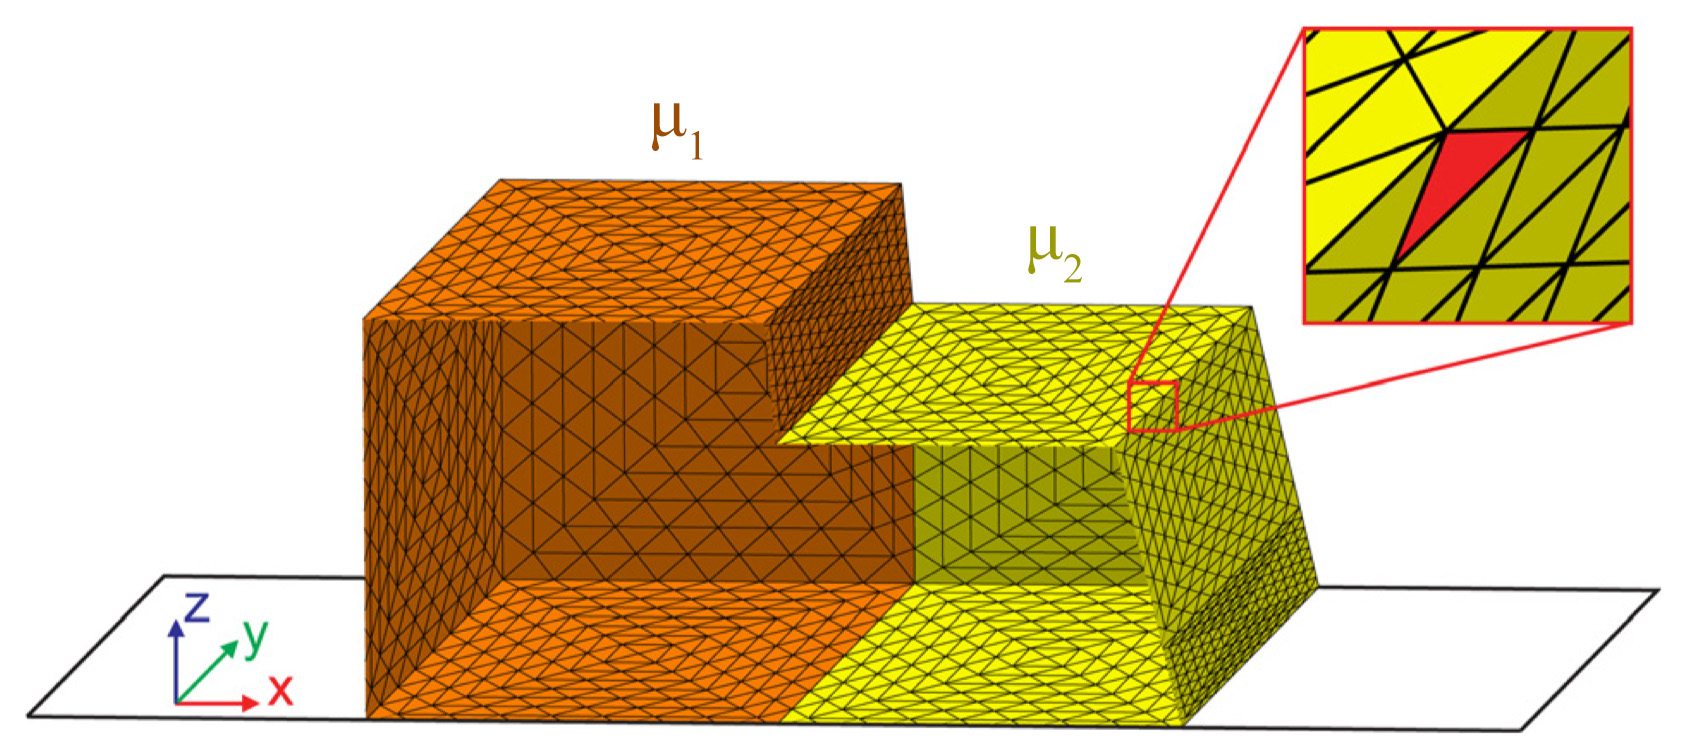
\includegraphics[width=0.9\linewidth]{SE_3}
		\caption{Модель поверхности образца, полученного методом полутоновой литографии, заданная в программе \textquotedbl Surface Evolver\textquotedbl{}~\cite{Kirchner_reflow}.}
		\label{fig:SE_3}
	\end{center}
\end{figure}






\section{Моделирование нагрева резиста при экспонировании}

Выделение энергии в резисте при экспонировании может приводить к повышению его температуры, что может повлиять на масштаб процессов, деполимеризации диффузии и растекания. Нагрев резиста при экспонировании будет рассматриваться для случая плоского слоя резиста, расположенного на поверхности полубесконечной подложки. В этом случае уравнение теплопроводности будет иметь вид~\cite{Cui_heating}:
\begin{equation} \label{eq:heat_diffusion}
	\begin{aligned}
		& \frac{\partial T_1}{\partial t}-k_1\left(\frac{\partial^2 T_1}{\partial x^2}+\frac{\partial^2 T_1}{\partial y^2}+\frac{\partial^2 T_1}{\partial z^2}\right) = h(x, y, z, t), \quad 0 < z \leqslant d, \\
		& \frac{\partial T_2}{\partial t}-k_2\left(\frac{\partial^2 T_2}{\partial x^2}+\frac{\partial^2 T_2}{\partial y^2}+\frac{\partial^2 T_2}{\partial z^2}\right) = h(x, y, z, t), \quad d \leqslant z < \infty,
	\end{aligned}
\end{equation}
где $d$ -- толщина слоя резиста, $k_i = D_i / \rho_i c_{v i}$ ($i=1,2$), $h=S / \rho c_{v}$. Здесь $D_i$, $\rho_i$ и $c_{v i}$  -- коэффициент теплопроводности, плотность и удельная теплоемкость резиста ($i=1$) или подложки ($i=2$). Величина $S$, определяющая скорость выделения тепла в резисте при экспонировании, может быть рассчитана по формуле
\begin{equation}
	S(x, y, z, t)=\frac{E_0 Q \lambda(\xi)}{R_{\mathrm{g}} t_{\mathrm{e}}},
\end{equation}
где $E_0$ -- энергия электронов в пучке, $Q$, $t_e$ -- доза и время экспонирования, соответственно, $R_g$ -- радиус Грюна:
\begin{equation}
	R_{\mathrm{g}}=\frac{4.6 \times 10^{-2}}{\rho} E_0^{1.75},
\end{equation}
а эмпирическая функция $\lambda(\xi)$ с параметрами $b_i$~\cite{Everhart_lambda} используется для определения энергии, выделившейся на глубине $z$:
\begin{equation}
	\begin{aligned}
	& \lambda(\xi)=b_0+b_1 \xi+b_2 \xi^2+b_3 \xi^3, \\
	& \xi=z/R_g.
	\end{aligned}
\end{equation}

\begin{figure}
	\centering
	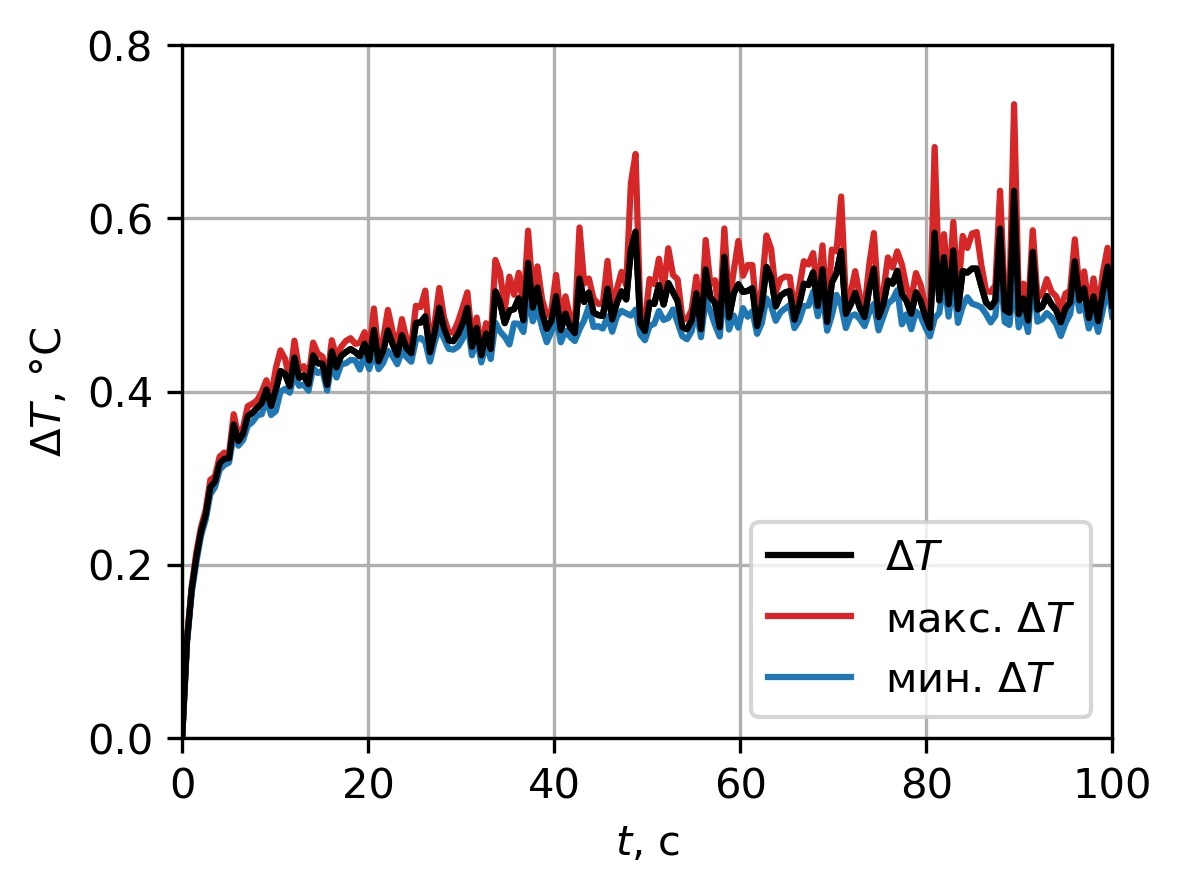
\includegraphics[width=0.7\linewidth]{heating}
	\caption{Система координат, используемая при моделировании нагрева резиста при экспонировании~\cite{Cui_heating}.}
	\label{fig:free_volume_diffusion}
\end{figure}

Граничные условия для уравнения~\ref{eq:heat_diffusion} имеют вид:
\begin{equation} \label{eq:heat_diff_eq_conditions}
	\begin{aligned}
		&\left.\frac{\partial T_1}{\partial z}\right|_{z=0} = 0, \\
		&D_1 \left.\frac{\partial T_1}{\partial z}\right|_{z=d} = D_2 \left.\frac{\partial T_2}{\partial z}\right|_{z=d}, \\
		&\left.T_1\right|_{z=d}=\left.T_1\right|_{z=d}, \\
		&\lim _{z \rightarrow \infty} T_2 = 0, \\
		&\lim _{(x,y) \rightarrow (\infty, \infty)} T_1 = \lim _{(x,y), \rightarrow (\infty, \infty)} T_2 = 0.
	\end{aligned}
\end{equation}

Решение уравнения~\ref{eq:heat_diffusion} с граничными условиями~\ref{eq:heat_diff_eq_conditions} выражается интегралом

\begin{equation}
	\begin{split}
		T(x, y, z, t) = & \int_0^{t_e} \mathrm{d} t^{\prime} \int_{-a / 2}^{a / 2} d x^{\prime} \int_{-b / 2}^{b / 2} d y^{\prime} \int_0^d h\left(x^{\prime}, y^{\prime}, z^{\prime}, t^{\prime}\right) \times \\ & \times G\left(x, x^{\prime}, y, y^{\prime}, z, z^{\prime}, t, t^{\prime}\right) d z^{\prime},
	\end{split}
\end{equation}
\begin{equation}
	G=\frac{1}{4 \pi k\left(t-t^{\prime}\right)} \exp \left(-\frac{\left(x-x^{\prime}\right)^2+\left(y-y^{\prime}\right)^2}{4 k\left(t-t^{\prime}\right)}\right) g,
\end{equation}
где для слоя резиста функция $g$ определяется выражением
\begin{equation}
	\begin{aligned}
		&g_1=\frac{1}{2 \sqrt{\pi k_1\left(t-t^{\prime}\right)}}\left[\exp \left(-\frac{\left(z-z^{\prime}\right)^2}{4 k_1\left(t-t^{\prime}\right)}\right)\right.+\exp \left(-\frac{\left(z+z^{\prime}\right)^2}{4 k_1\left(t-t^{\prime}\right)}\right)+\\
		&+\frac{2 \sigma K}{1+\sigma} \exp \left(-\frac{\left[d+z+K\left(d-z^{\prime}\right)\right]^2}{4 k_1\left(t-t^{\prime}\right)}\right)+\frac{2 \sigma K}{1+\sigma} \exp \left(-\frac{\left[d-z+K\left(d-z^{\prime}\right)\right]^2}{4 k_1\left(t-t^{\prime}\right)}\right)+\\
		&+\frac{2 \sigma K}{1+\sigma} \sum_{n=1}^{\infty}(-\alpha)^n \exp \left(-\frac{\left[(2 n+1) d+z+K\left(d-z^{\prime}\right)\right]^2}{4 k_1\left(t-t^{\prime}\right)}\right)+\\
		&+\frac{2 \sigma K}{1+\sigma} \sum_{n=1}^{\infty}(-\alpha)^n \exp \left(-\frac{\left[(2 n+1) d-z+K\left(d-z^{\prime}\right)\right]^2}{4 k_1\left(t-t^{\prime}\right)}\right)+\\
		&+\sum_{n=1}^{\infty}(-\alpha)^n \exp \left(-\frac{\left(z+z^{\prime}+2 n d\right)^2}{4 k_1\left(t-t^{\prime}\right)}\right)+\sum_{n=1}^{\infty}(-1)^n \alpha^{n-1} \exp \left(-\frac{\left(z-z^{\prime}+2 n d\right)^2}{4 k_1\left(t-t^{\prime}\right)}\right)+\\
		&+\sum_{n=1}^{\infty}(-1)^n \alpha^{n-1} \exp \left(-\frac{\left(2 n d-z^{\prime}-z\right)^2}{4 k_1\left(t-t^{\prime}\right)}\right)+\left.\sum_{n=1}^{\infty}(-\alpha)^n \exp \left(-\frac{\left(2 n d+z^{\prime}-z\right)^2}{4 k_1\left(t-t^{\prime}\right)}\right)\right]
	\end{aligned}
\end{equation}
и для подложки -- выражением
\begin{equation}
	\begin{aligned}
		g_2=& \frac{1}{2 \sqrt{\pi k_2\left(t-t^{\prime}\right)}}\left[(2-\eta) \exp \left(-\frac{\left(z-z^{\prime}\right)^2}{4 k_2\left(t-t^{\prime}\right)}\right)\right.-\\
		&-\eta\left(1+\frac{1}{\alpha}\right) \sum_{n=1}^{\infty}(-\alpha)^n \exp \left(-\frac{\left(2 n K^{\prime} d+z^{\prime}-z\right)^2}{4 k_2\left(t-t^{\prime}\right)}\right)+\\
		&+\beta \sum_{n=1}^{\infty}(-\alpha)^{n-1} \exp \left(-\frac{\left\{(z-d)-K^{\prime}\left[z^{\prime}+(2 n-1) d\right]\right\}^2}{4 k_2\left(t-t^{\prime}\right)}\right)-\\
		&-\beta \sum_{n=1}^{\infty}(-\alpha)^{n-1}\left.\exp \left(-\frac{\left\{(z-d)-K^{\prime}\left[z^{\prime}-(2 n+1) d\right]\right\}^2}{4 k_2\left(t-t^{\prime}\right)}\right)\right],
	\end{aligned}
\end{equation}
где
\begin{equation}
	\begin{aligned}
		&K=\sqrt{\frac{k_1}{k_2}}, \quad K^{\prime}=\frac{1}{K}, \quad \sigma=\frac{D_2}{D_1} \sqrt{\frac{k_1}{k_2}}, \alpha=\frac{\sigma+1}{\sigma-1},\\
		&\eta=\frac{2 \sigma K \theta}{1+\sigma}, \quad \beta=\frac{1+\alpha}{\sigma} \theta=\frac{D_1}{D_2} \frac{k_2}{k_1}.
	\end{aligned}
\end{equation}









